%%%%%%%%%%%%%%%%%%%%%%%%%%%%%%%%%%%%%%%%%%%%%%%%%%%%%%%%%%%%%%%%%%% 
%                                                                 %
%                            ROOT FILE                            %
%                                                                 %
%%%%%%%%%%%%%%%%%%%%%%%%%%%%%%%%%%%%%%%%%%%%%%%%%%%%%%%%%%%%%%%%%%% 
%
%  Run LaTeX or pdfLaTeX on this file to produce your thesis.
%  To produce the abstract title page followed by the abstract,
%  see the file abstitle-phd.tex or abstitle-mas.tex.
%
%%%%%%%%%%%%%%%%%%%%%%%%%%%%%%%%%%%%%%%%%%%%%%%%%%%%%%%%%%%%%%%%%%%
\documentclass[chap]{rpi_thesis}  
% Use the first command below if you want captions over 1 line indented. A side
% effect of this is to remove the use of bold for captions (thesis default).
% To restore bold, also include the second line below.
\usepackage[hang]{caption}      % to indent subsequent lines of captions
\renewcommand{\captionfont}{\bfseries} % bold caption (needed with caption 
                                       % package to restore boldface.)                       

\usepackage{subcaption}

\captionsetup[algorithm]{labelsep=colon}

\usepackage{graphics}
\usepackage{graphicx}
\usepackage{url} 
\urlstyle{rm}

% for eps diagrams
\usepackage{epstopdf}

% For algorithms
\usepackage{algpseudocode}
\usepackage[chapter]{algorithm}

\renewcommand{\algorithmicrequire}{\textbf{Input:}}
\renewcommand{\algorithmicensure}{\textbf{Output:}}

% For code
\usepackage{listings}
\renewcommand*{\lstlistlistingname}{LIST OF LISTINGS}

% For equations 
\usepackage{amsmath}
\usepackage{amsfonts}
\usepackage{amssymb}

\renewcommand{\vec}[1]{\mathbf{#1}}

% For tikz
\usepackage{tikz}
\usetikzlibrary{fit,positioning,shapes,arrows}
\pgfdeclarelayer{l1}
\pgfsetlayers{l1,main}
\makeatletter
\pgfkeys{%
  /tikz/node on layer/.code={
    \gdef\node@@on@layer{%
      \setbox\tikz@tempbox=\hbox\bgroup\pgfonlayer{#1}\unhbox\tikz@tempbox\endpgfonlayer\egroup}
    \aftergroup\node@on@layer
  },
  /tikz/end node on layer/.code={
    \endpgfonlayer\endgroup\endgroup
  }
}

\def\node@on@layer{\aftergroup\node@@on@layer}
\makeatother
% Define stage styles
\tikzstyle{stage} = [rectangle, draw, fill=blue!25, text centered, rounded corners, minimum height=2cm, inner sep=0.5cm, node on layer=l1]
\tikzstyle{substage} = [draw=blue,fill=white,dashed,rounded corners=0.25cm,align=flush center,text width=12em,inner sep=0.25cm,minimum height=1.5cm]
\tikzstyle{line} = [draw, -latex']
\tikzstyle{data} = [draw, rectangle, shape border rotate=90, aspect=0.25, fill=red!20, minimum height=2em, text centered]
\tikzstyle{decision} = [diamond, draw, fill=white, text width=4.5em, text badly centered, node distance=3cm, inner sep=0pt]
\newcommand{\nodebox}[2]{\parbox[c]{#1}{\centering #2}}

% For rotating in the tables
\usepackage{rotating} 
\usepackage[T1]{fontenc}

% To make the text tighter
% \usepackage{microtype}

% % For hyperreffing
\usepackage{hyperref}
% \usepackage[backref]{hyperref}
\hypersetup{
    unicode=false,          % non-Latin characters in Acrobats bookmarks
    pdftoolbar=true,        % show Acrobats toolbar?
    pdfmenubar=true,        % show Acrobats menu?
    pdffitwindow=true,      % page fit to window when opened
    pdftitle={My title},    % title
    pdfauthor={Author},     % author
    pdfsubject={Subject},   % subject of the document
    pdfnewwindow=true,      % links in new window
    pdfkeywords={keywords}, % list of keywords
    colorlinks=true,       % false: boxed links; true: colored links
    linkcolor=black,          % color of internal links
    citecolor=black,        % color of links to bibliography
    filecolor=black,      % color of file links
    urlcolor=black          % zcolor of external links
}
       
% TO CITE STUFF
\newcommand{\ignore}[1]{}
\newcommand{\nobibentry}[1]{{\let\nocite\ignore\bibentry{#1}}}
% apsrev entries in the text need definitions of these commands
\newcommand{\bibfnamefont}[1]{#1}
\newcommand{\bibnamefont}[1]{#1}
\newcommand{\Argmin}{\operatornamewithlimits{argmin}}
%\usepackage{natbib}
\usepackage{cite}
\usepackage{listings}
\usepackage{color}
\usepackage[toc,page]{appendix}
\usepackage{float}
\definecolor{dkgreen}{rgb}{0,0.6,0}
\definecolor{gray}{rgb}{0.5,0.5,0.5}
\definecolor{mauve}{rgb}{0.58,0,0.82}
\lstset{frame=tb,
  language=[Sharp]C, 
  aboveskip=3mm,
  belowskip=3mm,
  showstringspaces=false,
  columns=flexible,
  basicstyle={\small\ttfamily},
  numbers=none,
  numberstyle=\tiny\color{gray},
  keywordstyle=\color{blue},
  commentstyle=\color{dkgreen},
  stringstyle=\color{mauve},
  breaklines=true,
  breakatwhitespace=true
  tabsize=3
}

\renewcommand{\topfraction}{0.9}
\renewcommand{\bottomfraction}{0.8}

\setcounter{topnumber}{2}
\setcounter{bottomnumber}{2}
\setcounter{totalnumber}{4}

\renewcommand{\floatpagefraction}{0.8}


\begin{document}
% TO GET THE IEEE STANDARD RIGHT
%\bstctlcite{IEEE_Thing}
 
%%%%%%%%%%%%%%%%%%%%%%%%%%%%%%%%%%%%%%%%%%%%%%%%%%%%%%%%%%%%%%%%%%% 
%                                                                 %
%                            TITLE PAGE                           %
%               Master's Thesis or Master's Project               %
%                                                                 %
%%%%%%%%%%%%%%%%%%%%%%%%%%%%%%%%%%%%%%%%%%%%%%%%%%%%%%%%%%%%%%%%%%% 
%  This file produces the title page, copyright page (if requested)
%  and the Table of Contents, List of Figures and List of Tables.
% 
%  To produce the abstract title page followed by the abstract,
%  see the template file, "abstitle-mas.tex"
%%%%%%%%%%%%%%%%%%%%%%%%%%%%%%%%%%%%%%%%%%%%%%%%%%%%%%%%%%%%%%%%%%%

% Supply information for use on title page:    
\thesistitle{\bf Controller for Jumping Animations to Achieve Target Positions}
\author{Ian Charles Ooi}        
\degree{Master of Science} 
\department{Computer Science} % provide your area of study here; e.g.,
%  "Mechanical Engineering", "Nuclear Engineering", "Physics", etc.
   
\signaturelines{3}
\projadviser{Barbara Cutler} % For a masters project use \projadviser instead
%of \thadviser,
\memberone{Charles Stewart}        
\membertwo{Shawn Lawson}
%\memberthree{Aristotle} % must change signaturelines to 4 if using this 4 members

\submitdate{July 2015\\(For Graduation August 2015)}        
%\copyrightyear{2013}   % if omitted, current year is used.        

% Print titlepage and other prefatory material:   
\titlepage     
%\copyrightpage         %optional           
\tableofcontents        
\listoftables          %required if there are tables
\listoffigures         %required if there are figures
%\lstlistoflistings

   % titlepage material for Master's thesis or project
%%%%%%%%%%%%%%%%%%%%%%%%%%%%%%%%%%%%%%%%%%%%%%%%%%%%%%%%%%%%%%%%%%% 
%                                                                 %
%                         ACKNOWLEDGEMENT                         %
%                                                                 %
%%%%%%%%%%%%%%%%%%%%%%%%%%%%%%%%%%%%%%%%%%%%%%%%%%%%%%%%%%%%%%%%%%% 
 
\specialhead{ACKNOWLEDGMENT}
I would like to thank Rosa Tung and Jim McCarthy for acting as consultants for existing artistic methods as well as usage of tools which allowed me to produce the mesh and rig used in this thesis and showed me an artist's view of animation.  I would like to thank Jon Holman for discussing the mathematics of optimization problems with me, which helped to direct my choice for how to solve the problems.  Finally, thanks to my parents for their support and help with proofreading as well as sanity-checking my math.
%%%%%%%%%%%%%%%%%%%%%%%%%%%%%%%%%%%%%%%%%%%%%%%%%%%%%%%%%%%%%%%%%%%%
%                                                                 %
%                            ABSTRACT                             %
%                                                                 %
%%%%%%%%%%%%%%%%%%%%%%%%%%%%%%%%%%%%%%%%%%%%%%%%%%%%%%%%%%%%%%%%%%%

\specialhead{ABSTRACT}
Animating a character for video games and films is difficult and time consuming, requiring hours of artist labor to produce each animation.  These animations are set and inflexible, requiring changes to the animation or sometimes fully new animations to suit new characters or situations for natural looking movements.  Jumping is one such animation, where the size, mass, strength, and environment affect the movement of the character.  Traditionally these animations are produced by manually posing the character for certain key frames and interpolating between the frames to produce a smooth animation.  The more detailed or lengthy an animation, the more work required to specify it.  Physics-based simulation for animation production can reduce this work, creating animations for a variety of situations based on constants set for the character and environment.  These animations can then be easily recreated or adjusted for different environments by changing the constants set for generation.

This thesis work presents a simulation-based method of control for a character, focusing on the lower body, to produce jumping animations for a variety of situations and body parameters.  Two methods of simulation are described, one using a torque calculation and the other using an energy calculation to determine poses for the character.  My simulation takes as input a mesh representing the character, a tree of joints describing the skeleton, a set of muscles, mass assigned to each limb of the body, and a description of the desired path through desired timings, gravity, and desired displacement.  An inverse kinematic solver is used to aid in posing the character.

Contributions of this thesis include an implementation of a simulation to produce jump animations in \unity{}, a description of character poses based on torque as well as another based on energy, a sampling-based method for choosing a target position, and visualization of the produced animations in several ways to aid in debugging, analysis and presentation.

%When dealing with emergency situations in the wake of a disaster where the infrastructure of a region is damaged, a wide range of expertise is needed to quickly and efficiently solve issues. A prototype system for training emergency response personnel was designed to foster a collaborative environment through a single visualization with multiple users. The traditional methods of providing more detail in geographic data when dealing with a single user do not work in situations requiring interactions from multiple users, as this requires the loss of detail elsewhere within the fixed resolution of a display. The data being displayed in this simulation consists of a graph network of nodes and edges on top of a underlying series of satellite images. The nodes and edges are drawn over corresponding physical locations on the satellite images. When interacting with this system, it is often helpful to zoom in and increase the level of detail for two primary reasons: it is difficult to distinguish geographic features at low resolution, and subsequently, it is difficult to distinguish between nodes when the screen distance between them is relatively small. 

%This thesis work presents a method for providing a focus plus context solution to this system, allowing for continuous visual information with a minimal amount of distortion. This method creates circular areas of high magnification which gradually fall off to a base level surrounding individual cursors. These different regions achieve the original goals of zooming by providing a magnified look at the satellite images and increasing the screen distance between nodes. By having these regions centered on cursors, multiple users can view data on a shared display with their own degree of magnification while still retaining the ability to view the majority of the surrounding data.

%Contributions of this thesis include efficient implementations of rendering a graph network and text onto an underlying layer of satellite images, algorithms to perform the transformations of edges, vertices, and image data for rendering, and a preliminary feedback on the usability of these changes along with suggestions for a formal user study to be conducted as future work.
 	% abstract

%%%%%%%%%%%%%%%%%%%%%%%%%%%%%%%%%%%%%%%%%%%%%%%%%%%%%%%%%%%%%%%%%%% 
%                                                                 %
%                           INTRODUCTION                          %
%                                                                 %
%%%%%%%%%%%%%%%%%%%%%%%%%%%%%%%%%%%%%%%%%%%%%%%%%%%%%%%%%%%%%%%%%%% 
 
\chapter{INTRODUCTION}
\label{chapter:intro}

% magical first sentence
% explain like you would to your parents/non-technological people
% - explain how keyframe animation currently works
% explain in more technical terms what this means
% - problems with current techniques
% - what can be done (auto animation)
% - overview of controllers
% - overview of the technique
Animations of human characters are used heavily in video games, movies, and other fields.  Especially with the increasing usage of complex environment traversal in both film and video games, many similar animations of athletic motions must be created with small changes to tune the motion to the particular situation, environment, and character.  Creation of such animations is largely done by hand by artists using keyframing.  In a keyframe animation, certain ``key'' parts of the animated sequence are specified, with the remaining frames filled in, or ``tweened'' using an automated interpolation method or manual frame addition.  For 2D animation, this occurs as a series of images which are played back in order to produce the animation.  In 3D, keyframe animations are performed on a 3D model.

% figure of sprite animation frames
\begin{figure}[htp]
    \centering
    \includegraphics[width=\textwidth]{images/platformer_sprites_jump.png}
    \includegraphics[width=\textwidth]{images/platformer_sprites_walk.png}
    \caption[Example of a 2D Sprite Animation]{This example shows a 2D sprite sheet used to produce a jumping animation for a stick figure character.  The frames in this case are laid out in a single image for demonstration purposes, progressing in order starting with frame 0, the frame farthest left in this sprite sheet.}
\end{figure}

3D models are described as a mesh, a collection of primitive polygons (i.e. quadrilaterals or triangles) which are stored as vertices.  This mesh describes what is drawn, including any texture, color, and other material information.  Along with the mesh, a skeleton, or rig, is stored.  The rig describes a heirarchical structure of bones and accompanying joints.  Each vertex is given a series of weights describing the impact each joint has on its transformation.  This allows many vertices, and therefore many polygons, to be transformed at once in organized groups, simplifying the problem of animating the model to a matter of transforming the skeleton in the desired manner.  To animate this 3D model, an artist specifies keyframes of the animation by positioning the skeleton at different time steps.  The stored keyframes, instead of an image, are the transformations of each joint at this frame or step of the animation, which a rendering or game engine can interpolate between to produce the final result.

%TODO make the images the same level of zoom
\begin{figure}[htp]
	\centering
	\begin{subfigure}[b]{0.41\textwidth}
		\includegraphics[width=\textwidth]{images/simpleSkeleton2Screen1Cropped.png}
	\end{subfigure}
	\begin{subfigure}[b]{0.3\textwidth}
		\includegraphics[width=\textwidth]{images/simpleSkeleton2Screen2Cropped.png}
	\end{subfigure}
	\caption[Example of Rigged 3D Character Model]{Above is an example of a character model in AutoDesk Maya.  The character skin or mesh is shown in gray, with a rig shown in multicolor.  While it is visualized as a series of spherical joints with connecting solids, the rig itself does not have a visual component in practice.  The rig acts as a skeleton, deforming the mesh of the character model to make animation easier.  Additional tools such as deformer groups and inverse kinematics handles can be used to further simplify the creation of animations for artists.  While these tools simplify movement of the model, the artist still must position each joint for each frame of the animation, which is then stored for later playback.}
\end{figure}

Specifying these animation frames is work intensive, taking up significant time and resources to produce for a single character.  Additionally, similar animations may need to be produced for slightly different scenarios, with only minor modifications required.  These minor modifications can be to fit a different setting, such as a character jumping on Earth or on the moon, or can be for different characters, such as a large person moving in contrast with a small child.  Though the movement itself may be similar, manual changes must be made, requiring artist time which could be spent generating new assets.  

Recent work in animation generation seeks to automate this process, replacing the manual process with a procedural one.  Physics based simulations can be used to produce controllers for the skeleton, determining joint positions and rotations for keyframes automatically.  Not only does this reduce the effort involved in the creation process, but this also provides a basis for dynamic interaction between a character's animation and the environment, which is not possible with manual keyframe animations.

We present a controller that takes a skeleton as input, with additional parameters describing the character, which produces a sequence of poses for a keyframe animation.  The additional character parameters describe the character's mass as well as the constraints placed on each joint to prevent unnatural rotations.  Weight is specified per-joint to allow for calculation of the character's center of mass.  Our controller works with the initial flex and takeoff stage of the jumping motion.  The motion is calculated by modeling muscles as simple springs attached to the skeleton at 2 points.  Spring constants for the muscles are determined by the user, which are applied in a linear spring calculation to determine the approximate change from rest length required to achieve a particular force.  This change from rest length approximates the flexion required, which can be used to calculate a plausible amount of bend for the wind-up motion of a jump.

To control the motion and maintain plausibility, calculations are performed to determine the character's center of mass and supporting polygon.  As the character should maintain balance while flexing its joints, the position of the character's joints are adjusted to keep the center of mass positioned over the supporting polygon.  Flexion proceeds with the character bending progressively, maintaining balance while moving to achieve the desired spring force in its leg muscles.

The next stage of the motion, the take-off where the character releases from the ground, uses the potential energy of the spring-muscles and accelerates the character's center of mass upward.  Application of force works from the joints and muscles closest to the center of mass outwards through the skeleton.  While not handled by our controller, the character would then proceed through the in-air portion of the jump, where the acceleration changes due to gravity as well as other forces before they finally land.  We assume a simple trajectory for the in-air phase, though more complex motions with turns, flips, or interaction with the environment could be created.  Other work has handled landing with a similar approach. \cite{falling_landing}%TODO CITE karen liu

Our controller is made to be a module, able to be used with other controllers as part of a larger system.  This allows each controller to do a smaller job well. Several such controllers can be connected to produce more complex animations or animation sequences, utilizing bounded starting and finishing conditions for the character. Additionally, certain cases during the duration cause the controller to stop early, for example a mid-air collision mid jump which would require a separate controller to handle this case.%TODO CITE modular controllers

% figure of current keyframe animation process in maya
% accompanying video for presentation
% accompanying figure/video of the resulting animation in 3d

% explain contributions
% - what is the contribution of this technique
% - Unity3D -> what am I getting from outside sources
% - what am I making myself
\section{Contributions}
	This thesis describes a controller which simulates a jumping motion on a character.  The generated animation is created to be plausible in appearance, though it may not be a physically accurate representation.  Specifically, we contribute a model for the windup and take-off phases of a jump and created a controller using this model in Unity3D.

	Unity 3D is a game engine which we used to develop this system.  It provides infrastructure for rendering, scene management, skeletal animation, asset import and management, lighting, and scripting.  The system developed leverages the provided features through the Unity3D scripting interface.  We developed scripts for calculation of muscle forces, as well as for applying the force to an imported model.  Models were created in AutoDesk Maya and imported using Unity3D's asset import as Unity3D game objects with attached Transform components which allow arbitrary transformations.
 	% chapter 1

%%%%%%%%%%%%%%%%%%%%%%%%%%%%%%%%%%%%%%%%%%%%%%%%%%%%%%%%%%%%%%%%%%% 
%                                                                 %
%                           PREVIOUS WORK                         %
%                                                                 %
%%%%%%%%%%%%%%%%%%%%%%%%%%%%%%%%%%%%%%%%%%%%%%%%%%%%%%%%%%%%%%%%%%% 
 
% \specialhead{PREVIOUS WORK}
\chapter{PREVIOUS WORK}
\label{chapter:previous_work}

In this chapter, I will provide a more in-depth look at previous focus plus context systems and discuss the applicability of these techniques to our application.

\section{Focus Plus Context Visualizations}
\label{section:prev_fc_vis}

One of the earliest systems that tried to tackle the focus plus context problem was the \emph{Perspective Wall} presented by Mackinlay et al. \cite{Mackinlay1991}. This system was integrated with the \emph{Information Visualizer}, a system for visualizing data in 3D. The \emph{Perspective Wall} sought to imitate the nature of the human eye, by having a smooth integration between a focused area and the overall context. This system turns a 2D layout into a 3D wall system which contains
an area of detail surrounded by a distorted region. The \emph{Perspective Wall} had a flat region of high detail with regions surrounding it that were angled to match the field of view of the viewer. An image of the system is seen in Figure~\ref{fig:perspective_wall} showing the areas of magnification and demagnification. The focus of the application was to view information that was structured temporally, such as a filesystem. One of its greatest strengths was that it presented information in an intuitive manner. Unfortunately, while this work showed that such distortion techniques are helpful in facilitating understanding for the users, it is unsuited for our own purposes as this system performs a global distortion of the data and the metaphor does not easily extend to a system with different regions of focus.

\begin{figure}[htp] \centering
    \includegraphics[width=0.45\linewidth]{img/Perspective_Wall.jpg}
    \includegraphics[width=0.45\linewidth]{img/perspective_wall_actual.jpg}
    \caption[Perspective Wall Diagram]{A figure showing the magnified and demagnified regions of the 
        \emph{Perspective Wall} \cite{Mackinlay1991}, and an image of the original system, created by Mackinlay 
        et al.. The blue regions are demagnified and represent the angled areas.}
    \label{fig:perspective_wall}
\end{figure}

Baudisch et al.\ attempted to display focus plus context information through the integration of different hardware into a single logical screen \cite{Baudisch2001}. This screen consists of a low resolution region for context and a high resolution area for detailed information. They achieve similar effects as a fisheye view, but avoid distortion with their hardware. The prototype constructed integrates a LCD screen with a projection screen; a diagram of the system along with an image
of the actual system is seen in Figure~\ref{fig:f_and_c}.  By having two distinct regions of resolution, they are able to maintain the overall
geometry of the displayed images. To achieve this effect, Baudisch et al.\ created a foam core projection screen with a cutout for a flat panel LCD monitor. A large portion of the work performed by Baudisch et al.\ was used for examining this system with different applications. Of particular note is their work with a map application for finding the shortest path between two cities. The display allowed for seeing both the surrounding geography and large highways between the cities, while
allowing the user to also view street-level detail for areas with densely packed information. A single application controls the rendering for both screens. The data is rendered at a resolution that would fill the projection screen if it was also high resolution. A region is clipped to fit the resolution of the LCD monitor, while the overall data is scaled to fit within the projection screen. This solution provides a distortion free visualization, but only has a single area of
higher resolution. Viewing different regions of the data is performed by moving the entire visualization, which is not well suited to interactively viewing different areas simultaneously, but works perfectly fine for a single user. Generating new hardware is also outside of the scope of this thesis, but the studies performed by Baudisch et al.\ provide useful insight. In a small user survey, it was found that the overall responsiveness of the application as well as the ability to see the bigger picture of the work was beneficial for users of the system.

\begin{figure}[htp] \centering
    \includegraphics[width=0.45\linewidth]{img/f_and_c.jpg}
    \includegraphics[width=0.45\linewidth]{img/f_and_c_actual.jpg}
    \caption[Focus Plus Context Screen Diagram]{A figure showing the areas of high and low resolution images of 
    the focus plus context \cite{Baudisch2001} system created by Baudisch et al.. The red region is the LCD screen and the white area is the 
    projector screen.}
    \label{fig:f_and_c}
\end{figure}

Following their previous work, a formal study of the benefits of focus plus context displays was performed by Baudisch et al. Three different interfaces were evaluated with a number of different tasks to discover what display techniques were most helpful for completing said tasks \cite{Baudisch2002}. The focus plus context system described previously was compared with a zoom plus pan interface using a single screen and a overview plus detail interface using two monitors. All of the displays had approximately the same number of pixels between them. To further attempt to control for any extra space affecting the result of the experiment, the overview screen in the overview plus detail interface was constrained to the same size as the context of the focus plus context interface, while normally it would show the entirety of whatever dataset is being observed. There were two different types of tasks asked of the participants, the first was a static view where the users had to either
verify connections on a circuit board or find the closest hotel to a given point, and the second was a dynamic application where users were tasked with avoiding rocks and nails in a simple simulation. It was hypothesized and discovered that the focus plus context interface was the most helpful for performing both types of tasks. These results are promising for the infrastructure visualization, it suggests that a view providing a seamless integration between global and local data is most helpful in performing tasks which require both types of data. 

Gansner et al.\ describe a method for rendering sets of data with millions of nodes \cite{Gansner2005}. Their method, which they name ``Topological Fisheye'', follows the general principle given by Furnas et al.\ in  by having a detailed region around a focus with less information in other areas \cite{Furnas1986}. To reduce the amount of data in areas
out of focus, they create approximations of the original graph. When an area comes into focus, a hybrid graph is constructed by combining the various different approximations based on the distance from the focal point. To simplify the graph, they generate a proximity graph using either Delauney triangulation or a relative neighborhood graph and combine the results with the original edges of the graph to form a candidate set S. This set is then filtered by maximizing a weighted sum
of various measurements of the two points to be collapsed. The methods described in this construction are definitely applicable to future versions of the infrastructure visualization. As our data set grows, we may need to first simplify our graph data to filter out less important nodes. This filtered data could then be further transformed by a geometric transformation. A pure application of this would not adequately modify the underlying satellite images of our graph network.

\section{Geometric Transformations}
\label{section:prev_geometric_transformations}

As mentioned in Section~\ref{section:intro_fac}, the generalized fisheye view was described by Furnas in 1986 \cite{Furnas1986}. This method was later reworked in 1992 by Sarkar and Brown, who produced a method for performing geometric transformations to visually distort graphs and maps. This method changes the position, size, and level of detail based on the distance between the original object and the point of focus. An important distinction between this work and the generalized fisheye view is that the latter has objects either completely visible or not present at all, while this graphical method allows for a continuum \cite{Sarkar1992}.

Vertices are first positioned away from the focus via a transformation function. Given a vertex's original position, $P_{norm}$, the position of the focus, $P_{focus}$, and the max distance a vertex can move, $D_{max}$, the resulting fisheye position, $P_{feye}$ can be calculated.

\begin{equation}
    \label{eq:sarkar_fisheye} 
    P_{feye} = G(P_{norm})D_{max} + P_{focus}
\end{equation}

$G(P_{norm})$ is a monotonically increasing function that is continuous over the range $0 \leq x \leq 1$ with $G(0) = 0$ and $G(1) = 1$. 

\begin{equation}
    \label{eq:g_sarkar} 
    G(P_{norm}) = \frac{d + 1}{d + \frac{D_{max}}{D_{norm}}}
\end{equation}

In the above equation, $D_{norm}$ is the distance from the original point to the focal point, and $d$ is a distortion factor.

This general equation provides the basis for the transformations discussed later in Section~\ref{chapter:magnification}. The resulting new point of the transformation we apply to points should be based on the original location for the vertex and the location for a focal point. While Equation~\ref{eq:sarkar_fisheye} is helpful in creating a solution to our visualization problem, the distortion factor does not cleanly map to a degree of magnification. This distortion is helpful
for visualizing purely graph based data, but does not directly apply to magnification of images. When viewing a satellite image, being able to modify the magnification to any amount is important, as more detail is shown through this process. Graph based data does not need this type of magnification, as it only further increases the distance between elements.

Similar geometric transformations are discussed  by Kadmon and Shlomi\ for the distortion of maps with multiple focal regions \cite{Kadmon1978}. A similar basic function is given for transforming the scale of the map at a given point, \emph{P}, with a original scale $S_0$, the original distance from $P$ to the focus, $R$, and a distance function $f(R)$.

\begin{equation}
    \label{eq:kadmon_polyfocal} 
    S = S_0 + S_0 f(R)
\end{equation}

Unlike the equations created by Sarkar and Brown, Equation~\ref{eq:kadmon_polyfocal} is defined over the entire input. It exhibits similar behaviors in that the function $f(R)$ is chosen to cause $S$ to decrease as $R$ increases. Kadmon and Shlomi give the following general equation for $f(R)$.

\begin{equation}
    \label{eq:f_kadmon}
    f(R) = \frac{A}{1 + CR^2}
\end{equation}

The constant factors $A$ and $C$ represent the power of the focus and the rate of change, respectively. This pair of equations has a similar problem of constants which result in unclear transformations for the implementation. Being able to modify the scale to set amounts allows users to switch between views consistently and avoid confusion that would occur if the scale factor was not discrete steps. An additionally helpful insight from is that points which are affected by multiple
foci at the same time are affected by the sum of the individual foci \cite{Kadmon1978}. This insight is useful for the implementation of our own magnification functions when dealing with multiple areas of magnification.

The idea of magnification transformations is explored further by Keahey and Robertson. They propose the idea of combining linear and non-linear transformation functions to take advantage of the strengths of both. Linear functions are often desirable due to the fact that they perform zooming without introducing distortion into the system. This region of linear zoom can be important when trying to read text or other data that is sensitive to distortion. The non-linear region trades
distortion for the ability to fit more data in a smaller area. The resulting piecewise transformation allows a user to view a region in high detail while still retaining the context of the surrounding data. The application of this combination is seen in Figure~\ref{fig:regions_diagram}, which illustrates a region of linear magnification surrounded by a region of non-linear magnification

\begin{figure}[htp] \centering
    \includegraphics[width=0.8\linewidth]{img/regions_diagram.jpg}
    \caption[Combined Linear and Non-linear Magnification Regions]{An image of our infrastructure visualization magnification regions. The blue area is the non-linear magnification and the red region is the linear magnification. Note that despite being distorted, the roads in the image are still connected in both regions, allowing the user to trace a continuous path.}
    \label{fig:regions_diagram}
\end{figure}

Keahey and Robertson also note that performing such transformations on different domains has different requirements. When manipulating graph networks, the overall adjacency of nodes and edges is maintained for most transformations, linear or non-linear. Visual data requires more focus on the boundaries between the different transformation functions, as the boundary regions are especially susceptible to visual errors if they are not C0 continuous. An example image of a
magnification function that is not C0 continuous is seen in Figure~\ref{fig:non_continuous}. This resulting magnification includes a loss of data due to the discontinuity. These concerns are directly
applicable to designing a solution, as our data is stored in both a graph network and a series of satellite images. 

\begin{figure}[htp] \centering
    \includegraphics[width=0.3\linewidth]{img/non_continuous.jpg}
    \includegraphics[width=0.6\linewidth]{img/discontinuity_graph.jpg}
    \caption[Loss of Visual Data]{The magnification function for this transformation is not C0 continuous, and as such, causes a loss of data and discontinuities of geographic data.}
    \label{fig:non_continuous}
\end{figure}

In addition to discussing the relevant concerns of combining transformation functions, Keahey and Robertson describe a few methods for combining regions of magnification. Of particular note is his proposal for weighted averaging that simply transforms a point by all nearby functions and calculates weights as the inverse of the distance between the center of magnification and the original point. This method does not obscure data, and is simple to implement for our purposes

In this new paper, Keahey and Robertson generalize the non-linear magnification problem by removing the concept of foci \cite{Keahey1997}. They make a distinction between transformation and magnification, where the former indicates the distortion of the space, with the magnification function being the derivative of the transformation function. By generalizing the problem to a scalar field, we can derive the magnification of a particular element based on its own properties. Given a particular magnification mesh, computing a corresponding transformation grid is difficult, as it involves trying to convert a single magnification value into a two coordinate system. The solution presented uses an iterative method to approximate a numerical solution. The work done in is well suited to the task at hand for our data when either the satellite images or graph network are displayed
independently. However, we still need to create our own magnification functions to modify the underlying scalar field and create a region of linear zoom. This method simply removes the need for thinking about the magnification problem with regards to focal points. 

Keahey later generalizes the overall focus plus context problem into a detail plus context problem \cite{Keahey1998}. Up to this point, most focus context systems create focus by enlarging specific regions while compressing other regions. This does not inherently produce more detail within this region, as it simply makes the existing data easier to distinguish. He proposes a few different methods of adding detail to such regions like displaying different view levels. By
showing different view levels, the amount of information displayed in a region changes, as the original non-linear transformation merely causes a change in terms of size and shape. He mentions that this process could be used for map based data, and this technique is definitely helpful for future work (Chapter~\ref{chapter:future_work}).

In contrast to the fisheye visualizations of data presented by Kadmon and Shlomi, Sarkar and Brown, and Keahey and Robertson,  Elmqvist et al.\ present a method for folding space to achieve a focus plus context view \cite{Kadmon1978} \cite{Sarkar1992} \cite{Keahey1996} \cite{Elmqvist2010}. The other techniques present a visualization that is visually similar to a fisheye lens, focusing more on having a lot of global data. This method contextually folds 2D data into 3D such that
the only regions displayed are areas within focus. This devotes most of the screen space to the focal points at the cost of being able to see most of the global data. Where other techniques that utilize focus plus context expand the region around focal points, the system
created by Elmqvist et al.\, M\'{e}lange, compresses the
unimportant areas of the display. A diagram of this system is seen in Figure~\ref{fig:melange}, notice that the red region, corresponding to the magnified areas, take up the majority of the display. Relative distance between focal points within the distorted region is represented by a number of folds, each indicating a complete screen distance. While this method produces interesting results, it is important in our visualization to have a majority of the information undistorted. M\'{e}lange focuses on showing as much detail around the focal points as possible, but the goals for a visualization of our system are to show a smaller area of increased focus while maintaining as much context as possible.

\begin{figure}[htp] \centering
    \includegraphics[width=0.45\linewidth]{img/Melange.jpg}
    \includegraphics[width=0.45\linewidth]{img/melange_actual.jpg}
    \caption[M\'{e}lange Diagram]{An image comparing magnified and demagnified regions of the M\'{e}lange system 
    \cite{Elmqvist2010}, developed by Elmqvist et al.\ as well as the system applied to a visualization of an   
    adjacency diagram.}
    \label{fig:melange}
\end{figure}

B\"{o}ttger et al.\ present a method for manipulating a distorted city map to highlight specific areas of interest in \cite{Bottger2008}. The motivation for this system was the combination of geographic data and a stylized subway network to display more information around areas on the stylized network diagram. They introduce a concept called \emph{Warping Zoom}. Given a set of control points, they create a mapping function which moves any number of control points to other positions.
These individual control points correspond to the different subway stops and routes on the original mapping and are moved to positions to form the stylized network. While this method would allow for the separation of clustered data within our visualization by warping the overall data, it does not provide a solution for viewing the satellite data at a higher level of detail, nor does it perform an easily classifiable magnification function. To perform a magnification of a region of
satellite images, the system would have to define multiple control points and their resulting position. This is essentially performing the same transformation as a simple magnification function, but only focuses on manipulating a few points. 

\section{Summary}
\label{section:PREVIOUS_WORK_SUMMARY}

This chapter provided an overview of works which attempt to use a focus plus context visualization. I discussed a variety of applications which focused on utilizing some sort of focus plus context solution to solve their visualization issues. Finally, applications and research which concerned geometric distortions of data were summarized with respect to our goals. The following chapter discusses the changes performed to our visualization to improve performance and allow for implementation of our magnification function.

%%%%%%%%%%%%%%%%%%%%%%%%%%%%%%%%%%%%%%%%%%%%%%%%%%%%%%%%%%%%%%%%%%% 
%                                                                 %
%                             Animation                           %
%                                                                 %
%%%%%%%%%%%%%%%%%%%%%%%%%%%%%%%%%%%%%%%%%%%%%%%%%%%%%%%%%%%%%%%%%%% 
 
\chapter{ANIMATION}
\label{chapter:animation}

Jumping is the acceleration of a character's center of mass upward.  This motion can be divided into several stages.  First is the lead-up or wind-up stage in which the character flexes or gathers momentum to perform the jump.  This takes the form of a slight crouch (TODO reference cat jumping paper or the background .  should this be in background?) which prepares the character to exert the necessary force against the ground.  

Next comes the take-off stage.  The character pushes against the floor with their feet, accelerating their center of mass to break contact with the floor.  

\section{Setup and Inputs}
%TODO should this just be in the animation section?
The character in our system consists of a mesh, a skeleton, and a controller which has itself several sub-components.  First we constructed a mesh, a 3D visual representation of our character.  Our mesh is a simple, blocky humanoid, lacking arms in order to focus more heavily on the lower body motion of the figure.  A more complex human character, or even a humanoid non-human character could be substituted.  This mesh consists of vertices, which each have a position as well as other information not relevant to our simulation such as normal and texture coordinate, which are used by \unity for displaying the mesh.  This mesh can also be referred to as a character model, but in the context of this simulation we will refer to it as the mesh.  Three vertices form a triangular face, though these are often created as quadrilaterals by the artist as the topology of the model can be simpler to work with due to the grid patterns formed as compared to triangular meshes.  In the case of quad meshes, the mesh is often treated as a triangle mesh by the game engine or renderer, with each quad producing two triangles.

Our mesh was created using \maya, positioning the vertices in groups or individually, using several rectangular prisms as a base.  Using the edge loop tool, more vertices were inserted, with loops of edges circling the torso and legs to produce the final shape.  This mesh was then rigged, meaning a skeleton was added.  As described in further detail in \ref{subsection:skel_joints}, joints were positioned individually relative to the mesh, attempting to mimic the positioning of joints in the human skeleton.  The connections were made simply, with each joint acting as a ball and socket joint, meaning that constraints needed to be specified at a later stage to facilitate hinge joints such as the knee and ankle and that complex, multi-boned structures as found in the foot and shin were simplified to a single bone connecting two joints.  The hierarchy of joints for the skeleton was rooted at the pelvis with three children: one leading to the upper body and one to each hip.  From there a single joint was used for the manipulation of the upper body, with separate joints for each hip, knee, ankle, toe, and heel.  Though there is no movement in the toe, placing a bone for the foot requires an end joint for the bone to connect to.

%TODO how do i talk about this with authority, there isn't really anything to cite there's just youtube videos and it's generally taught as such/discovered via industry
Joints are then associated with the mesh through weight painting, in which each vertex of the mesh is assigned a weight for each joint.  This weight designates if and how much a vertex transforms when a joint is moved.  Each vertex must be assigned a weight for each joint of the model.  Careful weight assignment is highly important as this determines the behavior of the character's ``skin'' when they move, affecting how the mesh twists or bends as well as which parts move with which bones.  The joints may then be used to manipulate the mesh to produce animations, with each keyframe in an animation storing information about each joint instead of each vertex.

\subsection{User Specified Constants}
\label{subsection:user_constants}
% specified constants
% gravity
% air time
% windup time
% error allowance (between calculated skeleton values and desired)
% drag
% jumping policy (not implemented)
% Windup PD k values
% Balance PD k values
% muscle values foreach muscle:
%	k (linear spring constant)
%	anchor joints (for our simulation, 2)
% 	center joint
%   [0,1] scale to indicate muscle anchor position (0 is closer to center joint, 1 is closer to end joint)
%   bone width
% calculated values
Within the controller there are a number of constants the user can specify, outside of the character itself.  These specify constants for the simulation environment as well as some constants describing the animation to be produced.  Our only environmental constant is gravity, which we specify as -10 $\frac{m}{s^2}$, where the negative indicates the downward direction.  Other constants include the air time, windup time, error allowance, and constants for the PID controllers.

The times indicate how much time the character is expected to spend in the air and winding up for the jump.  Air time in our case consists of the portion of the animation where the character's feet are not in contact with the ground plane.  Windup time refers to the time in which the character has their feet on the ground and is in the process of accelerating their mass upwards as the initial takeoff portion of the jump.  A long windup time gives a very slow, exaggerated jumping motion while a short windup gives a very rapid, clipped motion.  While we allow the user to specify any time for both air and windup, in practice there is a limited range of values that are possible for the character.

%TODO example windup times with our chosen values

\subsection{Skeleton, Joints, and Muscles}
\label{subsection:skel_joints}
For the purposes of animation, a joint is an object with an associated position, associated transformation, a parent joint, and some number of child joints.  In the case of the root, the parent joint is absent and in the case of the end joints such as tips of the fingers there are no child joints.  Each child joint is connected to the parent by a rigid bone, which protrudes from the parent at a given resting angle.  These joints are structured in a tree, as the parent and child joints imply, with the root of the tree at the pelvis.  This tree serves as a hierarchy for transformations.

Joints are associated with a set of vertices from the mesh to be animated.  Each of these may be associated with multiple joints, and are assigned a weight for each joint which acts as a scale factor for the transformations performed on the vertex.  When a joint is transformed, the transformation is propagated to the children, with the parent as the origin of the child node's coordinate system.


%%%%%%%%%%%%%%%%%%%%%%%%%%%%%%%%%%%%%%%%%%%%%%%
%               Torque Method                 %
%%%%%%%%%%%%%%%%%%%%%%%%%%%%%%%%%%%%%%%%%%%%%%%
\section{Torque-based simulation}
One method of simulation we attempted used springs placed along the length of each limbs to produce a torque on the joints of the character.  This method failed for unknown reasons.  Torques on the joints results from the force of the muscle pulling a bone to rotate about the joint, resulting in a complex system of motion with each bone rotating around the joints.  These rotations combine to move the body in a direction, allowing a character's control to be centered around degree and timing of muscle activation. \cite{muscle_based_bipeds}  In our case, we take the muscle as fully activated, which means that it has a spring constant defining the strength of the muscle.  This muscle is then stretched to produce the desired torque by bending the affected limb.  The restoring force of the spring-muscles produce torques which are used to calculate angular momentum, and from that linear momentum.  

\subsection{Path Estimation}

\begin{figure}[ht]
	\centering
	\begin{tikzpicture}[node distance = 1em, auto]
% Path Estimate Phase
	%	Path Estimate Stage
    \node [stage] (path) {\nodebox{10em}{Path Estimate \[a = \dfrac{2 (x - x_0 - v_0 t)}{t^2} \]}};
    %	Path Estimate Data
    \node [data, above of=path] (xf) {\nodebox{4em}{Target Position ($x$)}};
    \node [data, left of=xf] (xi) {\nodebox{4em}{Initial Position ($x_0$)}};
    \node [data, left of=xi](t){\nodebox{4em}{Time ($t$)}};
    \node [data, right of=xf] (vi) {\nodebox{4em}{Initial Velocity ($v_0$)}};
    \node [data, below of=path] (accel) {\nodebox{6em}{Target Acceleration ($a$)}};
    
    \path [line] (xi) |- (path);
    \path [line] (xf) -- (path);
    \path [line] (t) |- (path);
    \path [line] (vi) |- (path);
    \path [line] (path) -- (accel);
\end{tikzpicture}
	\caption[Diagram of path estimation algorithm]{Diagram of the path estimation step.}
	\label{fig:pathEstimate}
\end{figure}

\begin{figure}[ht]
	\label{fig:pathExample}
	\caption[Example of estimated path]{Example of a path estimation.}
\end{figure}
Before calculations relating to the model's skeleton are performed, an initial estimate of the jump path is performed.  The estimate uses a simple forward kinematic calculation to determine the force required to move an object through the air from the initial position of the model, denoted as $x_0$ in Figure \ref{fig:pathEstimate}, to a final position, denoted as $x$.  To facilitate a character jumping while moving, the path estimate takes into account the initial velocity $v_0$.

The user specifies a desired time ($t$), which indicates the time the character will spend airborne during the animation, i.e. the time between when the character's feet break contact with the ground and when they regain contact with the ground.  This is useful as the desired animation can be more easily adjusted to fit a desired time as an in-game animation or to fit a particular storyboard for an animated film sequence.

\subsection{Windup}
From this force, the acceleration can be determined using $F=ma$ from classical mechanics.  This assumes the character is a rigid body with negligible air resistance acted upon by gravity of $10\frac{m}{s}$.  The mass is calculated as the summed total of the distributed masses assigned to the character's limbs, which are summed to produce a total mass for the character.

Proportional derivative control is used to produce the windup motion once the initial path estimate is calculated.  The error function $E_{all}$ calculates error from the desired force $E_{force}$ as well as the balance $E_{balance}$.

Once computed, error is compared to a threshold ($\epsilon$).  If the error is below the threshold, the skeleton is considered bent to the proper position for windup and the system proceeds to the thrust phase in which the character unbends.  If the value is above the threshold, a new position for the hip is calculated using proportional-derivative control, where the new position for the iteration of the controller, $u(i)$, is calculated as \[u(i) = k_p E_{all}(i - 1) + k_d(E_{all}(i-1) - E_{all}(i-2))\] where $i$ is the iteration, and $k_p$ and $k_d$ are weights which determine the rate of change. This new hip position is given to an inverse kinematics component to calculate the positions of the remaining leg joints, assuming the feet should remain in the same position.  These new joint positions and angles are then passed back to the PD controller to re-calculate the center of mass as well as the new force and balance errors for the next iteration.

\begin{figure}[ht]
	\centering
	\resizebox{\textwidth}{!}{
		\begin{tikzpicture}[node distance = 0.5cm, auto]
% Bend Phase
    % before controller, need to calculate the desired 
    % place nodes
    \node [data, below of=path] (accel) {\nodebox{2.5cm}{Target Acceleration ($a$)}};
	\node [data, left=of accel] (mass) {\nodebox{3.5cm}{Body Mass assigned to each limb ($\left\lbrace m_0, \ldots, m_n\right\rbrace$)}};
    \node [stage, below= of accel] (forceCalc) {\nodebox{6cm}{Calculate desired force $F_{target} = \displaystyle\sum_{j=0}^n {m_j} a$}};
    % connecting lines
    \path [line] (accel) -- (forceCalc);
    \path [line] (mass) |- (forceCalc);
    % ----------------
	
    % PD controller
    % place nodes
    \node [substage, below=4cm of forceCalc] (bendErr) {Calculate error from desired force magnitude ($E_{force}$)};
    \node [substage, left=2.5cm of bendErr] (bendBal) {Calculate balance error ($E_{balance}$)};
    \node [substage, above=of bendBal] (comCalc) {\nodebox{5cm}{Calculate Center of Mass \[C_{mass} = \displaystyle\sum_{\forall m} m \cdot position(m)\]}};
    \node [data, below left=1cm and -2cm of bendErr] (bendErrAll) {\nodebox{4cm}{$E_{all} = E_{force} + E_{balance}$}};
    \node [decision, below=0.5cm of bendErrAll] (bendPDTest) {$E_{all} \overset{?}{\le} \epsilon$};
    \node [substage, left=1cm of bendPDTest] (bendPDEq) {Set new hip position based on $u(i) = k_p E_{all}(i) + k_d \left(E_{all}(i) - E_{all}(i-1)\right)$};
    \node [stage, label={[shift={(-0.5cm, 2cm)}, rotate=90]180:\LARGE PD Controller}, fit=(comCalc) (bendErr) (bendBal) (bendErrAll) (bendPDEq) (bendPDTest)] (bendPD) {};
    \node [data, below=2cm of bendPDTest] (bentSkel) {\nodebox{3cm}{Skeleton in bent position ($\theta_{x} \forall x \in J_m$)}};
    \node [data, below=1cm of bendPDEq] (bendPDConst) {
    \nodebox{4cm}{Proportional and Derivative weights ($k_p, k_d$)}};
    % connecting lines
	\path [line] (forceCalc) -- (bendErr);
	\path [line] (comCalc) -- (bendBal);
	\path [line] (bendErr) |- (bendErrAll);
    \path [line] (bendBal) |- (bendErrAll);
    \path [line] (bendErrAll) -- (bendPDTest);
    \path [line] (bendPDTest) -- (bendPDEq);
    \path [line] (bendPDTest) -- (bentSkel);
    \path [line] (bendPDConst) -- (bendPDEq);
    % ----------------
    
    % CoM inputs
    % place nodes
    \node [data, above =2cm of comCalc] (skeleton) {\nodebox{3cm}{Model with skeleton attached ($J = \left\lbrace j_0, \ldots, j_n \right\rbrace$, contains at least a pelvis and both left and right hips, knees, ankles, heels, and toes)}}; 
    \node [data, left=2cm of skeleton] (mjoints){\nodebox{7cm}{Muscled joints ($J_m = \lbrace$ $j_{pelvis}$, $j_{Lhip}$, $j_{Rhip}$, $j_{Lknee}$, $j_{Rknee}$, $j_{Lankle}$, $j_{Rankle}$, $j_{Lheel}$, $j_{Rheel}$, $j_{Ltoe}$, $j_{Rtoe}$ $\rbrace$}};
    \node [data, left=2cm of mjoints] (muscles) {\nodebox{7cm}{Muscle spring constant for muscled joints ($\left\lbrace k_0, \ldots, k_11\right\rbrace$)}};
	\node [data, left=2cm of muscles] (jconst) {\nodebox{5cm}{Rotation constraints for joints ($\theta_{min}, \theta_{max}$ $\forall j \in J_{muscled}$)}};
	
	% connecting lines
	\path [line] (skeleton) -- (comCalc);
	\path [line] (mjoints) |- (comCalc);
	\path [line] (muscles) |- (comCalc);
	\path [line] (jconst) |- (comCalc);
	% ----------------	
	
	% IK solver side stage
	% place nodes
	\node [data, left=6cmof bendPDEq] (IKCurJoint) {\nodebox{8cm}{$R = position(j)$ $\forall j \in J_{ik} \subseteq J$ starting with the root (hip joint).}};
	\node [data, left=3cm of IKCurJoint] (IKTargetPos) {\nodebox{8cm}{Target position for joint, in this case keeping $E$ in it's original position ($D$).}};
	\node [data, left=3cm of IKTargetPos] (IKEndJoint) {\nodebox{4cm}{Joint to move to target ($E$).}};
	\node [data, above=2cm of IKCurJoint] (IKRD) {\nodebox{6cm}{Normalized vector $\vec{RD}$}};
	\node [data, above=2cm of IKEndJoint] (IKRE) {\nodebox{6cm}{Normalized vector $\vec{RE}$}};
`	\node [substage, above=8cm of IKTargetPos] (IKEq) {$\theta_j = \vec{RD} \times \vec{RE}$.};
	\node [data, above left=3cm of IKEq] (IKItrs) {\nodebox{6cm}{Number of iterations for IK solver ($num_itr$)}};
	\node [data, left=29cm of comCalc] (IKPartBent) {\nodebox{5cm}{Bent skeleton reflecting $u(i)$.}};
	\node [stage, label={[shift={(-1cm, 5.5cm)}, rotate=90]180:\LARGE IK Solver}, fit=(IKCurJoint) (IKEndJoint) (IKTargetPos) (IKItrs) (IKRD) (IKEq) (IKPartBent)] (bendIK) {Requires joints to be in a single chain.};
    % connecting lines
    \path [line] (bendPDEq) -- (IKCurJoint);
    \path [line] (IKPartBent) -- ++(25cm, 0cm) -- ++(0cm, -4.5cm) -| (bendErr);
    \path [line] (IKPartBent) -- (comCalc);
    \path [line] (IKCurJoint) -- (IKRD);
    \path [line] (IKEndJoint) -- (IKRE);
    \path [line] (IKTargetPos) |- (IKRD);
    \path [line] (IKTargetPos) |- (IKRE);
    \path [line] (IKRD) |- (IKEq);
    \path [line] (IKRE) |- (IKEq);
    \path [line] (IKEq) -- (IKPartBent);
    \path [line] (IKItrs) |- (IKEq);
    % ----------------
\end{tikzpicture}
	}
	\caption[Diagram of windup phase algorithm]{Algorithm diagram of the windup phase.}
	\label{fig:bendPhase}
	%TODO decision lines need to be labeled
\end{figure}

\begin{table}[ht]
	\centering
	\caption[Table of PD controller constants for windup phase]{Example values for the PD controller constants, showing the sweet spot that we use as well as the effect of going higher or lower (how do we show this effect, show that the steps are too large or too small? time or iterations to finish?).}
	\label{tab:windup_pd_vals}
\end{table}

\subsubsection{Force calculation}
%TODO force calculation should be done with error in net torque instead of error in force as we don't really have a resultant force here and the net force really means nothing
% calculation of the muscle flexion
\begin{figure}[ht]
	\centering
	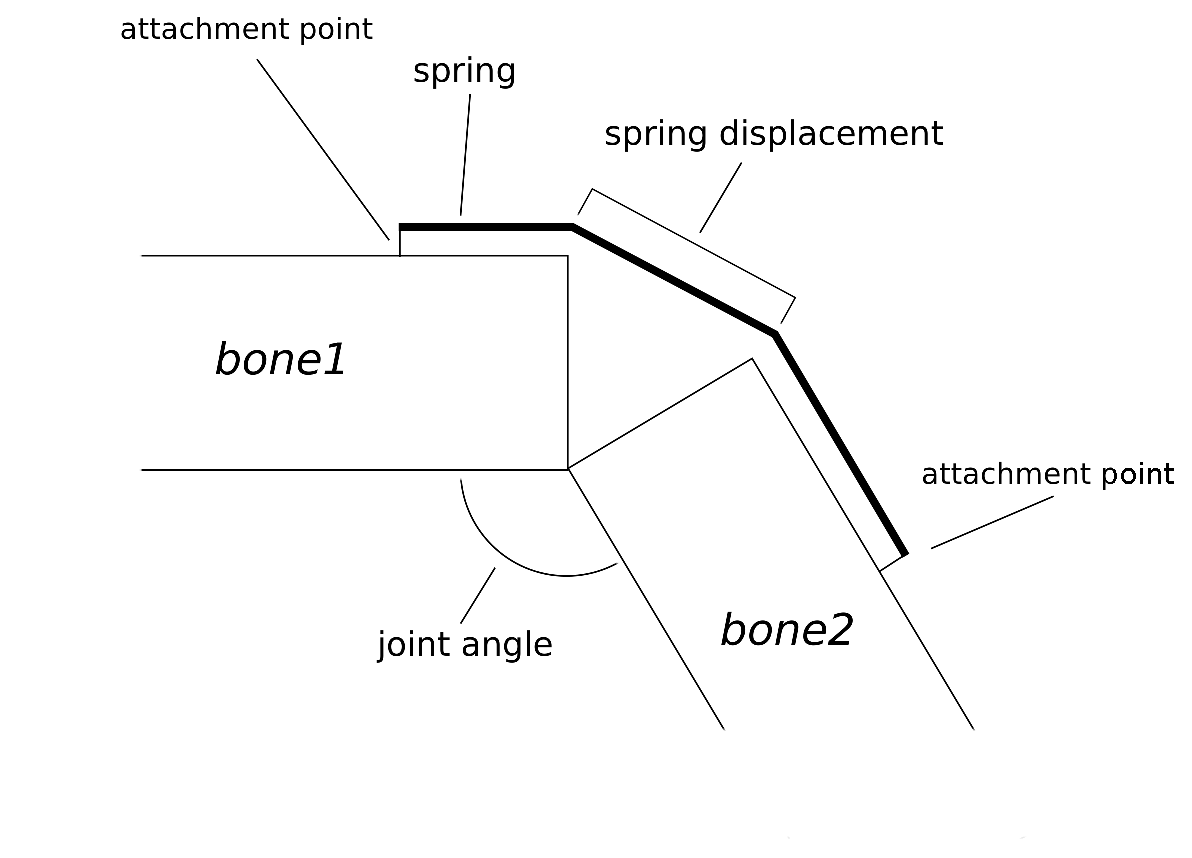
\includegraphics[width=10cm]{images/spring_calc/spring_angle_calc.eps}
	\caption[Diagram of joint force calculation]{Force calculation for a joint.}
	\label{fig:forceCalc}
\end{figure}
Current force is computed by approximating muscles as linear springs attached to two bones and crossing a joint.  The change in spring length is produced by the bend of the joint which opens a space between the rigid bones that the spring must stretch across.  This approximation uses spring constants that simulate a flexed muscle that has been stretched by an amount equal to \[\theta = cos^{-1} \left( \dfrac{2 k^2 r^2}{F^2} - 1 \right)\] which requires a more rigid spring constant.  In this equation, $r$, represents the width of the bone, which is a constant that changes the amount the character must bend to achieve a force.  This acts similarly to the $k$ value, which represents the stiffness of the spring, or a constant for the linear restoring force of the muscle.  
%TODO For our simulations, we used values in the range ().
%TODO values and equation
%TODO tables of values with varied k and varied r and corresponding bend/angle
\begin{table}[ht]
	\centering
	\caption[Table of spring muscle constants]{A table of various values for k and r, demonstrating effect on the model's bend.  TODO Columns of k and r (varied individually), and image of fully bent character resulting from values.}
	\label{tab:variedSpringValues}
\end{table}

At each iteration of the PD controller, current force output of the legs is computed.  An accurate calculation of the force must take into account the torques ($\vec{\tau}$) produced by the muscles on each joint.  We use a simplified version, calculating the magnitudes of the torques which avoids the complexity of implementation and computation.  This is found for a joint j as \[\tau_j = ||\vec{r_j}|| F_j\] where r is the moment arm, the cross product between the vector between the attachment point of muscle and the center of the joint with the direction of the muscle crossing the joint.  Direction of a muscle is in the direction of restoration of the spring (TODO double check this, is this always the value we want, point placed along the spring based on the masses on each end) as used in \cite{muscle_based_bipeds}.
%TODO does this setup effectively result in springs connected in series? No because you can assume that the muscles you don't want to unbend with remain rigid?
%TODO does this give a sort of impulse function as you unbend at the hips and knees, then the ankles?
%TODO this is where the torques come into play, and they're absolutely necessary

\begin{figure}[ht]
	\centering
	\caption[Algorithm diagram for calculation of force error]{Force error calculation}
	\label{fig:forceErr}
\end{figure}

To calculate the error used for PD control, the vector between the two forces is measured, indicating the change required in both direction and magnitude.  As we require the force to act in the direction of acceleration, the main adjustment is the force magnitude.  When instead considering the torque magnitude, the magnitude alone can be considered. (TODO I think I need to be using the torque magnitude instead of a force here).

\subsubsection{Center of Mass and Balance}
%TODO need to standardize usage of joint to anatomical, animation, or something else
The center of mass (CoM) is calculated as the centroid of the character.  More specifically, joint positions are averaged, with a weight assigned to each joint based on the weight of the limb associated.  The CoM must be recalculated with each update to the character's pose as the shift in weight changes the position.

Using the calculated CoM, the balance of the character can be determined by the position of the CoM relative to the supporting polygon of the character.  The supporting polygon is a polygon determined by the points of contact of the character with the ground or other supports which provide a normal force to counteract gravity and other external forces.  During the windup and thrust phases, the character maintains contact with the ground through their feet, with the outer edges of the feet forming two sides of a quad, a line between the two feet at the toes forming a third, and a line between the heels of the character forming the fourth side.  This polygon should be parallel to the ground plane, and is positioned at the bottom of the feet.  If the character's center of mass is over this supporting polygon, the character is balanced.

\begin{figure}[ht]
	\centering
	\caption[Algorithm diagram for calculation of balance error]{Balance error calculation.}
	\label{fig:balanceErr}
\end{figure}

To quantify balance, the vector between the center of the supporting polygon and the position of the CoM is measured.  This vector is then projected into the same plane as the supporting polygon, giving a 2 dimensional error between where the CoM is currently and where it would need to be to be perfectly centered.  The PD controller then attempts to minimize the magnitude of this vector by moving in the proscribed direction while bending to achieve the desired force, constraining the number of solutions possible to provide the desired force.
% does the vertical distance have effect?  you're going to fall over more easily if you're on a stilt as opposed to crouching over your feet as the moment will be (bigger? is that bigger?).  the lever will be more able to move your weight easily

\subsubsection{Inverse Kinematic Solving}
As the skeleton is a hierarchy assumed to be rooted at the hip, a problem arises with applying rotations to joints.  To keep a character's feet rooted to the floor as is expected, positions must be solved for using inverse kinematics.  Given the desired position for the hip, and the desired position of the foot, the joint angles and positions of the knee and ankle are solved for.  Constraints are placed on each joint, limiting the range of motion to an expected range as well as limiting the axes about which each joint can rotate, preventing unnatural directions of motion.  These values are specified per joint and can be edited by the user to simulate varied levels of flexibility or alternate body shapes.

%TODO alternate body with digitigrade, Tauren or whatever from WoW, raptor style...
%TODO Further justification of why choosing this method instead of learning is that this is more user-tunable as opposed to a learning heavy model which doesn't allow as much user tuning

\begin{table}[ht]
	\centering
	\caption[Table of joint constraints]{Joint angle constraint values used for each joint, with accompanying images of expected motion range.}
	\label{tab:jointConstraints}
\end{table}

A solution to the joint positions is found using these constraints, and gradient descent method which works on single-chains of joints.  A single chain of joints is a sequence of joints in which each joint has a single child and a single parent, with one root joint and one leaf joint which lack a parent and child respectively.  Given the hierarchy of joints and a desired position for one of the non-root nodes of the chain, cyclic-coordinate descent (CCD) is used to determine rotations of the joints between the joint in question and the root that will minimize the distance between the joint in question and the desired position.  This algorithm is shown in \ref{alg:ik}.

\begin{algorithm}[ht]
	\centering
	\begin{algorithmic}[H]
		\Function{SingleChainIK}{C, D, E}
		\Repeat
		\ForAll{Joints R between E and the root, starting with the end E}
			\State $\theta_R = \vec{RD} \times \vec{RE}$
		\EndFor
		\Until{\textit{Desired number of iterations performed} or \textbf{E} \textit{is close enough to} \textbf{D}}
		\EndFunction
	\end{algorithmic}
	\caption[Single chain IK algorithm]{Given chain of joints C, move joint E to position D using cyclic coordinate descent (TODO cite CCD references).  This process iteratively moves joint E closer to the location D, concentrating on each joint R in the chain one at a time and solving the geometric problem of minimizing distance between E and D by rotating R.}
	\label{alg:ik}
\end{algorithm}

This approach, while for the specific case of single chains of joints, is simpler to implement than other approaches such as the pseudo-inverse of the Jacobian.  In addition, this approach allows some flexibility, specifically in constraints of the joints.  As each joint is addressed individually instead of the system as a whole, any constraints placed on the joint can easily be accounted for by simply preventing the joint from rotating out of the desired range while the rest of the system continues to move as close as possible to the solution.  One downside is that a halting condition must be determined, through a minimum acceptable distance.  To handle the case where the joint cannot be moved within this minimum distance, a maximum number of iterations must be designated.  In practice, 100 iterations is enough to converge, with as few as 30 working well for our simulation.

\subsection{Thrust and Takeoff}
\label{subsection:thrust}
Upward acceleration is animated by calculating the angular accelerations of the joints given the forces acting upon them and the resulting torques.  Torque is the change in angular momentum over time, allowing for the acceleration to be calculated as the mass can be assumed to be constant: \[\tau = \dfrac{dL}{dt} = m \dfrac{dv_{\theta}}{dt} = m a_{\theta}\] where $\tau$ is the torque of a joint, $L$ is the angular momentum, $m$ is the mass of the limb, which must take into account the mass of the rest of the body which is also moved by the limb, $v_{\theta}$ is the angular velocity and $a_{\theta}$ is the angular acceleration. This results in the below equation for determining angular acceleration. \[a_{\theta} = \dfrac{\tau}{m}\]

Using angular acceleration, the intermediary poses for the model can be determined at each timestep.   For each frame, an explicit Euler integration is performed to determine first angular velocity and finally angle.  As the character continues to extend, a check is made for if the character has yet reached full extension.  At full extension, the character can no longer accelerate in the direction of the jump, and the character breaks contact with the ground to enter the in-air phase.

\subsection{Sampling}
To determine which of numerous possible solutions is the most desirable, we take several samples.  A sample is described by the position of the pelvis joint, the resulting linear momentum, and a vector describing the displacement of the character's center of mass from the center of its support to indicate balance as described above.

Samples were restricted to a box defined by a rectangle around the character's feet with a height reaching the position of the character's pelvis when standing at rest.  Any sample outside of this volume is assumed to put the character off balance.  Samples were then taken at uniformly distributed positions in this region.  The calculated acceleration was projected onto the desired acceleration vector through the dot product, with values greater than or equal to the desired acceleration's magnitude indicating a plausible solution.  These plausible solutions are then ordered by their balance error, calculated as the difference in position between the center of mass and the center of the supporting polygon.  The first result of this list is then chosen as the candidate answer and the pelvis is moved towards this sample.  At each iteration this is repeated until the desired acceleration is achieved.
%To select the minimum sample, the collected data were organized first by the difference between the linear momentum calculated and the desired linear momentum, and the top ten percent were selected.  Ten percent was found empirically to be a good selection of points to select the most balanced from while also retrieving points with very low differences from the desired.

\subsection{Rebalancing}
As the character re-positions its pelvis, the balance must be calculated again and its position accordingly re-adjusted.  To maintain the position of the legs, we use the upper body to achieve balance.  A separate PD controller is used to regulate the rate of movement.  While the character shifts its balance to achieve a particular acceleration, it bends its upper body, moving the weight forward, backward, left, or right to attempt to center itself over its supporting polygon.

%%%%%%%%%%%%%%%%%%%%%%%%%%%%%%%%%%%%%%%
%               Energy                %
%%%%%%%%%%%%%%%%%%%%%%%%%%%%%%%%%%%%%%%
\section{Energy Based Calculation}
Another way we considered using for simulation was energy based.  We assumed that the energy required to lift the mass of the character and move it the necessary distance is equivalent to the summed elastic potential energies of the leg muscles.  The direction of the velocity is determined by the direction the center of mass is accelerated after the windup phase, and we assume that this is achievable given that the character can achieve the desired energy.  Change in direction is achieved through usage of the feet and shift of weight during the acceleration and windup phases.  If a character wishes to move forward, they shift their weight back farther during windup, allowing them to accelerate forward farther before becoming airborne.

As with the torque-based simulation, the jump follows the stages of path estimation, windup, thrust, in-air, and landing.  Thrust and in-air follow the same method as described in \ref{subsection:thrust}, so we describe the path estimation and windup below.

\subsection{Path Estimation}
Kinetic energy is calculated as \[ E_k = \frac{1}{2} m v^2 \] where $m$ is the mass of the character and $v$ is the velocity.  Mass remains constant, and velocity can be calculated by 
%Given that work is the change in kinetic energy, velocity
%\begin{align*}
%	W &= F d \\
%	&= \delta E \\
%	&= \frac{1}{2} m \left(v^2 - v_0^2\right)
%\end{align*}

\subsection{Solutions to the Energy Assignment Problem}
The setup of the problem resembles a quadratic programming problem.  In this problem, we minimize: \[ \vec{x}^T \mathbf{Q} \vec{x} \] subject to
\[ \vec{x}^T \mathbf{P} \vec{x} \le r \] where $x \in R^6$ and $\mathbf{Q}$ and $\mathbf{P}$ are square, $6 \times 6$ matrices.  $\mathbf{Q}$ for our problem is a diagonal matrix, where the diagonals contain the spring constants $\left\lbrace k_1, k_2, ... , k_6 \right\rbrace$ and $\mathbf{P}$ is $- \mathbf{Q}$.  We can introduce additional constraints in the form of maximum and minimum values for all $x_i \in \vec{x}$, where the minimum and maximum are calculated at the minimum and maximum rotations of the joint, producing the extremes in spring displacement.

This problem of quadratically constrained quadratic programming is NP-hard and as such we sought a simpler problem or approximation to solve to obtain a solution.  As with the torque method, we choose a sampling-based approach as there is a known limit on the possible solutions in our case: balance.  Like with the torque-based method, sampling took place in the region where the character maintains balance.  Samples were collected at regular intervals within a bounding box defined by the character's supporting polygon, the ground, and the the height of the character's pelvis at full extension.  The pelvis was repositioned and the resulting elastic potential energy measured.
\section{Summary}
\label{subsection:animation_summary}
%
%%%%%%%%%%%%%%%%%%%%%%%%%%%%%%%%%%%%%%%%%%%%%%%%%%%%%%%%%%%%%%%%%%% 
%                                                                 %
%                           METHODS                               %
%                                                                 %
%%%%%%%%%%%%%%%%%%%%%%%%%%%%%%%%%%%%%%%%%%%%%%%%%%%%%%%%%%%%%%%%%%% 
 
% \specialhead{METHODS}
\chapter{VISUALIZATION}
\label{chapter:visualization}
In this chapter I discuss methods of visualization for the animations produced in Chapter \ref{chapter:animation}, as well as the difficulty of visualizing character animation in print format as well as video.  I present some sources of inspiration for my visualizations and motivate the need for visualizations.  I then discuss techniques I utilized to visualize my data for presentation as well as for debugging and analysis.

% talk about instpiriations here instead of prev work
\section{Motivation and Inspiration}
\label{section:vis_insp}
Showing a motion in a static medium such as print presents numerous challenges.  The static image or images must convey a sense of time that is understandable, such that a viewer may intuit the direction and rate of movement.  Especially for a complex object such as a figure, occlusion can obstruct information, and prevent understanding of the motion of hidden portions of the body.  The projection of a 3D scene can also create similar issues as occlusion, creating ambiguity in depth and obscuring motions in some dimensions.

I drew from several sources for inspiration on how to visualize my results.  A video by KORB created for the CCTV Documentary Channel shows ``motion sculptures,'' in which the people in the scene leave trails of material as they move\footnote{https://vimeo.com/69948148 [Accessed: Nov. 23, 2015]}.  These sculptures very cleverly captured the movement of the body throughout the space of the video, creating aesthetically pleasing, if somewhat difficult to parse, visuals.

Another film of a similar nature is Choros by Michael Langan and Terah Maher \footnote{http://langanfilms.com/choros.html [Accessed November 18, 2015]}.  Images of a single dancer follow her through her her movements, leaving a traceable pattern of movement.  This technique was inspired by chronophotography, a precursor to video which utilizes multiple successive photographs or multiple exposures on the same film to visualize movement of a figure or object.  These can be laid out in animation strips or superimposed to create a single image.

\section{Motion Visualization}
\label{section:motion_vis}
%For visualizing motion of a character or figure, there are a limited selection of different techniques.  Most common is a sequence of frames in which a character is posed, either in a still sequence or as a video.  As this is a final goal of my system, this is a valid visualization, but fails to provide a simple comparison between one animated sequence and another.  This is desirable for qualifying or quantifying performance of the system.  A sequence of still images is also space-consuming, which can be undesirable for print formats or even digital formats where length or size of document is an issue.

Markers were used to highlight motion of particular parts of the body, such as the pelvis or center of mass.  Other indicators placed on or around the figure can indicate other values, such as arrows to represent vectors of force.  This however can result in clutter within the images, scene, or frame of video, occluding or distraction from the primary animation.  Copies of the character could be left behind to produce an after image effect such as in the videos discussed in section \ref{section:vis_insp}.  I used these techniques in conjunction with each other, enabling and disabling them as the situation required.


\begin{figure}[ht]
	\centering
	\includegraphics[width=\textwidth]{images/trails/trail-side.png}
	\caption[Marker trail visualization of motion]{An example of the markers tracking joints.  With a high sample rate, a curve forms trailing along the path of the joint.  Markers were placed at a rate of 10 per second of simulation time.}
	\label{fig:marker_trails}
\end{figure}

Markers were implemented as camera-facing ``billboard'' planes with a texture that were spawned with a user-specified frequency, following an arbitrary joint of the character.  Each frame the orientation of the planes adjusts such that it faces the main active camera, allowing very little geometry to be used to produce an always visible visual to be placed in the scene.  I used one of these for each joint in the legs as well as one for the pelvis in order to track the paths of the joints.  This visualization was an interesting one to view, and gave a similar effect to motion sculptures, but was very difficult to understand without a reference to know which color of marker corresponded to which joint.  Even with knowledge of which joint followed which trail of markers, the visualization was difficult to understand, though it gave a good overview of the whole motion.  These marker trails are shown in Figure \ref{fig:marker_trails}.

\begin{figure}[ht]
	\centering
	\begin{subfigure}[b]{0.49\textwidth}
		\includegraphics[width=\textwidth]{images/ghosts/side-sparse.png}
	\end{subfigure}
	\begin{subfigure}[b]{0.49\textwidth}
		\includegraphics[width=\textwidth]{images/ghosts/side-dense.png}
	\end{subfigure}
	\caption[Ghost image visualization]{Pictured above are examples of a ghost image visualization achieved by placing copies of the character model at a rate of 1 per 0.5s (pictured left) and 1 per 0.2s (pictured right).}
	\label{fig:ghost_vis}
\end{figure}

I used a ghost image visualization as well in 2 ways: leaving copies of the character behind at a user defined rate and layering collected frame data.  In the first method, I make a copy of only the model and necessary skeleton components, leaving out the extra data such as mass, constraints, and muscles used in my simulation, and match the positions and rotations of each of its joints to the character at the current time.  The ghosts use a semi-transparent material to help differentiate between them and the model, as well as to provide some clarity as to each ghost's pose and combat the issues of occlusion.  Examples of this visualization are shown in Figure \ref{fig:ghost_vis}.

\begin{figure}[ht]
	\centering
	\includegraphics[width=\textwidth]{images/k200kvaryingcomposite.png}
	\caption[Composite frame visualization]{An example of the composited frames visualization, in which several frames of the animation are layered on top of each other, and matte painted to produce a combined image with all frames superimposed.}
	\label{fig:composite_vis}
\end{figure}

An alternate method of forming the ghost image visualization was to layer numerous collected frames in an image editing program.  This method was very work intensive, requiring each layer to be matte painted by hand.  Algorithms and techniques in image processing and computer vision for automating this process, but for my purposes it was necessary to manually select the desired region in each image that should be visible in the final combined image.  To reduce the negative effects of occlusion, layers above the first were given an opacity of $75\%$.  Though work intensive, this produced an excellent visual for still media to show the path of the entire motion, but was a poor visual in many cases for showing detail of the movement as images often occlude each other.  Examples of this visualization are shown in Figure \ref{fig:composite_vis} and in Figure \ref{fig:complex_scene}.  As a compliment to this visual, I used animation strips, in which the frames were simply presented adjacent to each other in order from left to right.  These strips are also found in the data tables presented in Section \ref{section:image_results} and in Figure \ref{fig:complex_scene}.

\section{Debugging Visualizations and Controls}
\label{section:debug_control_vis}

For debugging visuals, I used a feature in \unity{} called Gizmos \footnote{http://docs.unity3d.com/ScriptReference/Gizmos.html [Accessed: August 10, 2015]}, which allowed debug drawing of primitive shapes.  I used small spheres of various colors to show sample positions, target positions for the IK solver, corners of the supporting polygon, and the position of the center of mass.  Rays were used to visualize velocity, acceleration, distance to the destination, and value of the samples.  A screenshot of my Gizmos active for an energy based simulation are shown in Figure \ref{fig:gizmo_vis}.

\begin{figure}[ht]
	\centering
	\begin{subfigure}[b]{0.49\textwidth}
		\includegraphics[width=\textwidth]{images/handles1.png}
	\end{subfigure}
	\begin{subfigure}[b]{0.49\textwidth}
		\includegraphics[width=\textwidth]{images/handles2.png}
	\end{subfigure}
	\caption[Screenshot of Handles used for setting and visualizing joint constraints in \unity{}]{Screenshots of Handles, a tool in \unity{} which allows the user to create custom UI elements in the editor for changing a value in the game or simulation.  In this case, the Handles affect the minimum and maximum rotation for the joints.  Handles are only visible when the corresponding object is selected by the user, reducing clutter.  All three Handles are shown in the left image, allowing the user to set the constraints for pitch (red), yaw (green), and roll (blue) as the pelvis is set to allow rotations about all three axes.  At right, I show the Handle for adjusting the constraints of the left knee, which is only able to rotate about the x-axis (pitch).}
	\label{fig:handle_vis}
\end{figure}

Similar to the Gizmos, I utilized a feature called Handles \footnote{http://docs.unity3d.com/ScriptReference/Handles.html [Accessed August 13, 2015]} to ease setting and visualization of the joint constraints on the skeleton.  Unlike a Gizmo, a Handle can be manipulated by the user to affect values in the simulation before run time.  As shown in Figure \ref{fig:handle_vis}, three handles were used to adjust pitch, yaw, and roll, color coded as red, green, and blue.  Colors were chosen to correspond to the colors of the reference axes placed in the scene to aid the user, showing the red, green, and blue handles as limiting rotation about the x, y, and z axes respectively.

\begin{figure}[ht]
	\centering
	\begin{subfigure}[b]{0.49\textwidth}
		\includegraphics[width=\textwidth]{images/gizmos1.png}
	\end{subfigure}
	\begin{subfigure}[b]{0.49\textwidth}
		\includegraphics[width=\textwidth]{images/gizmos2.png}
	\end{subfigure}
	\par\medskip
	\begin{subfigure}[b]{0.49\textwidth}
		\includegraphics[width=\textwidth]{images/gizmos3.png}
	\end{subfigure}
	\begin{subfigure}[b]{0.49\textwidth}
		\includegraphics[width=\textwidth]{images/gizmos4.png}
	\end{subfigure}
	\caption[Screenshot of Gizmos used for debug visualizations in \unity{}]{Screenshots of Gizmos in the \unity{} Editor.  The green points illustrate the sample field taken at the beginning of the jump, while the gray lines show the energy measured at this sample.  The rays beginning at the player's pelvis show the magnitude and direction of the acceleration (magenta) and velocity (blue) of the character.  The green line at the player's feet shows the displacement from the start position to the destination, and the cyan line starting at the player's pelvis shows the calculated kinetic energy.  At right, a closer view of the samples is shown to show the blue dots which outline the balanced region which the samples were restricted to.  The character is distanced from these samples as the Gizmos are drawn at the character's start position, and the character in this scene has completed its jump and is at the destination position.  The orange particle is a marker placed at the start position.}
	\label{fig:gizmo_vis}
\end{figure}

\section{Discussion}
\label{section:vis_discussion}
The hope for the visualizations was to provide simple, at-a-glance diagnostics that would show an animation's strengths and shortcomings.  Tracking individual joints with markers provided surprisingly little information, though I had hoped it would provide a simplified way of looking at the overall motion of the character, eliminating unnecessary visuals of the character model and providing information purely about the skeleton.  While less useful than I had hoped, the trails following the joints did provide information about the general path of the character, though detail was often obscured by overlapping portions of the trail. One such case was where the character's foot was becoming trapped in the ground and ended up twisting in place, instead of remaining stationary as a support.  The twisting trail around the foot joint provided a simple visual that there was movement where there should not be.  This visualization also indicated that the information provided by the character model is necessary to understanding the animation of the character, leading to the ghost image visualization.

The ghost image visualization provided similar information, but kept the character model.   Due to the regular sampling of the character's position, this visualization was good for finding temporal issues, where the character spent too great or too small a time in different portions of the jump.  One such instance was that the character had an issue where the inverse kinematic solver could not keep up with the rate at which the character moved when performing the windup animation for a ``superman'' jump, in which the muscles were tuned such that the character could jump to the top of a 200m block.  The motions occurred too quickly due to the large values involved, necessitating a finer timestep so that the simulation would not overshoot.  This visualization showed the back-and-forth adjustments occurring due to the simulation constantly passing the target pose by over-adjusting.

The Gizmo visuals were used out of necessity.  The dots were inserted in order to visualize the samples and the values that each produced, as the output animations for early iterations were very far from expected motions and the animation itself provided very little information about the target or calculated values.  These visualizations helped to find mathematical errors in the torque-based simulation, as well as leading to the abandonment of the torque-based simulation in favor of the energy-based simulation when the values of the torque-based simulation remained very far from expected, but the energy-based simulation produced similar values to those expected.  The gizmos were also used to visualize the balance of the character, showing center of mass and the supporting polygon.

Handles were used as a utility, as setting the angle constraints on the joints of the character was a long and difficult process, with very little to indicate if the range was ``realistic'' or ``expected.'' The angles in \unity{} are not always as expected, since a rest angle of the joint may be $0^\circ$, while biologically the rest angle may be defined as $180^\circ$.  Handles provided a way to have not only a visual representation of the constraints on the joints, but also a more intuitive method of entering them.  Instead of typing in the numbers in the \unity{} Inspector, the Handles may be dragged to modify the values.  Creating Handles for the specification of muscles would likely make the process of setting up the skeleton much easier and more intuitive for animators, and is of high priority for future iterations of this system.

\section{Summary}
In this chapter I discussed some difficulties in visualizing animations in both animated and non-animated settings.  I presented some sources of inspiration and discussed the different methods I used to visualize data for presentation, analysis, and debugging.  Methods I used for analysis and presentation included trails of markers, ghost images created by duplicating the player model in the scene, layering frames to create a single image, and animation strips.  My debugging visualizations took advantage of \unity{} utilities, using Gizmos and Handles to allow the user to see information about the simulation, as well as to more easily adjust constraints on the skeleton.
\label{section:vis_summary}

%\include{Validation}

%%%%%%%%%%%%%%%%%%%%%%%%%%%%%%%%%%%%%%%%%%%%%%%%%%%%%%%%%%%%%%%%%%% 
%                                                                 %
%                           RESULTS                               %
%                                                                 %
%%%%%%%%%%%%%%%%%%%%%%%%%%%%%%%%%%%%%%%%%%%%%%%%%%%%%%%%%%%%%%%%%%% 
 
% \specialhead{INTRODUCTION}
\chapter{RESULTS}
\label{chapter:results}
In this chapter we discuss results of our simulation.  First in Section \ref{section:pd_constants_results}, we describe choosing of the constants for the proportional derivative controllers, which required proportional ($k_p$) and derivative ($k_d$) constants to control the rate at which changes were applied to the simulation, motivating the choice of values in Table \ref{tab:pd_constants}.  We then discuss choice of muscle strength constants, as well as the length and height of trial jumps in Section \ref{section:muscle_results}.  This section also gives an estimate for how strong a human leg with similar dimensions would be.  Section \ref{section:speed_frame_results} describes performance of the simulation as well as our method of collecting frame data.  Examples of this collected frame data is shown in Section \ref{section:image_results}.  Finally, we discuss limitations of our simulation and method in Section \ref{section:limitations}.

\section{Proportional Derivative Controller Constants}
\label{section:pd_constants_results}
The windup PD controller was given constants of $k_p = 0.25$ and $k_d = 0.25$.  These were chosen empirically to offset irregularities due to time step and slow convergence in the inverse kinematic solver.  With higher values, the translation of the pelvis results in the character's feet embedding in the ground plane due to too great a movement in a single frame.  The feet then fail to adjust as the inverse kinematic solver cannot converge quickly enough.  As opposed to a performance issue, this is a limitation of the inverse kinematics algorithm used, which was chosen due to simplicity so focus of this project could remain on the jump simulation.  

In most cases, the inverse kinematic solver converged within 30 iterations, but in this situation more than 300 iterations were required.  To compensate, we chose PD controller constants to adjust the rate of of change of the animation.  These values were found to generally produce smooth windup phases without compromising on speed of the animation too much, where speed refers to the amount of movement in each frame, which requires the frames to be played back at a different rate to achieve the desired rate of movement in the final animation.

The controller for re-balancing performed well with $k_p = k_d = 1$, with little noticeable change in results and only a change in rate of convergence for values at $k_p = k_d = 0.5$ and $k_p = k_d = 1.5$.  This showed that the main bottleneck for control in the model was the windup control, leading us to choose the value 1.

\section{Muscle Constants and Strength Intuition}
\label{section:muscle_results}
Muscle spring constants were tested in various configurations, with several trials run for each set of constants for varying distances, directions, and situations.  Animations were created for forward jumps between 1m and 2m for the normal human values and at 1m, 10m, and 100m for the super human, based on the analysis of the standing long jump by Wu et al\cite{longjump}.  A jump onto a box was also simulated, with 0.5m and 0.75m boxes for the normal human and 1m and 100m boxes for the super human.  The normal human muscle constants were additionally used for sideways jumping animations, as well as a more complex scene in which the character is made to jump from on top of a box, over an obstacle before finally landing on the ground.

%biomechanics of sport and exercise
Jump animations appear plausible, and the spring values result in forces similar to a human muscle.  Human muscles have about $30\frac{N}{cm^2}$ force per cross-sectional area\cite{biomech_sport}. We perform the following calculation as an intuitive estimation of the expected leg strength of the character. The character's leg thickness is about $0.20m$ forward to back narrowing towards the knee, with a left-right thickness of around $0.15m$. If we assume that skin is about $0.002m$ thick (2mm) and about $15\%$ of the remainder is subcutaneous fat, we are left with a $0.1683m$ by $0.1258m$ cross section.  This gives an axial cross sectional area of approximately $0.021m^2$.  We use a bone width of $0.05m$, giving a cross sectional bone area of $0.0025m^2$ which leaves an area of $0.019m^2$ of non-bone muscle.  If half of this is extensor muscle, then we have an approximate cross sectional area of $0.0095m^2$ or $95cm^2$.  This means that the estimated maximum isometric force for the muscle is $F = \left(30 \frac{N}{cm^2}\right) \left(95cm^2\right) = 2850N$.  With a $k$ of 20000, our muscle produces \[
	F = -k \left(\dfrac{r \sin (\pi - \theta)}{\sin \frac{\theta}{2}} \right)
\]
which for a joint bend of $\frac{\pi}{2}$ radians is $1414N$.  A more accurate $k$ value for the single muscle would be $40000$ but $20000$ suffices as the smaller muscles of the calf are modeled as overly strong.  The $k$ value was determined empirically, following the assumption that an average person has a max long jump in the range of 1.5m to 2m.  A possible explanation is that our simulated character can perfectly execute the movement, maintaining balance and applying force.  There is a non-trivial technical aspect to performing a jump, meaning that a human with the capability to perform a longer jump may not be capable of maximizing their range due to imperfect technique.
%  The character in our simulation has a femur length of 0.4m and a shin length of 0.33m.  Our muscle crossing the knee has anchor points set between the knee and the ankle, and the knee and hip.  These anchors are set at $0.2 * 0.33m = 0.066m$ and $0.9 * 0.4m = 0.36m$ respectively, where $0.2$ and $0.9$ are values in $[0,1]$ which indicate how far along the bone the anchor is set as described in \ref{subsection:skel_joints}.  This gives a total length for this muscle as $0.426m$ or $42.6cm$. 

The produced animations are plausible and recognizable as jump animations.  The character loads its limbs appropriately, giving the appearance of weight, and extends its knees, hips, and lastly ankles to show thrust corresponding to the usage of its muscles.  As in a real jump, the character extends its ankles last, the calf muscle providing the final thrust of the motion.


\section{Simulation Speed and Frame Collection}
\label{section:speed_frame_results}
The simulation runs in an interactive frame rate, with a delay on start up for the calculation of the sample field.  As long as the mass and the muscle constants remain the same, the sample field need not be re-calculated.  The sample field calculation is linear in the number of samples taken.  A major bottleneck aside from populating the sample field is the convergence of the inverse kinematic solver.  The solver is guaranteed to run every frame, usually for many iterations unless it has already converged.  While the cost is manageable due to the linear nature of the algorithm, the main issue is when convergence does not occur and the simulation must either stop and wait for the solver to catch up, or continue on and risk corrupting the simulation due to misplaced joints or limbs.  There are two major cases of this occurring: the character's feet sinking into the ground instead of the knees bending during windup and the character's feet prematurely breaking contact with the ground during thrust.  Our simulation suspends its activities when a compromising situation is detected, iterating the inverse kinematic solver until the issue is resolved.  The solver usually converges within a few frames, but this can add undesired time to the simulation and undesired frames to the animation.

Frame data was collected at a rate of 1 frame per 0.1s of simulation time, giving a frame rate of 10 frames per second.  This granularity was used to ensure capture of any irregularities in the simulation and to ensure changes in pose were recorded as shorter trials ran in under 1s of simulation time, though the real time was several seconds.  Finer granularity was found to have little benefit.  We show one of five frames in the tables discussed in section \ref{section:image_results} to reduce the size of the animation strips presented and thereby reduce the size of our tables.

\begin{table}[ht]
	\centering
	\scriptsize
	\begin{tabular}{| c | c | c | c | c | c | c |}
		\hline
		& Left Hip & Left Knee & Left Ankle & Right Hip & Right Knee & Right Ankle \\ \hline
		Global, Normal & 20000 & 20000 & 20000 & 20000 & 20000 & 20000 \\ \hline
		Varying, Normal & 20000 & 24000 & 16000 & 20000 & 24000 & 16000 \\ \hline
		Uneven Global, Normal & 16000 & 16000 & 16000 & 24000 & 24000 & 24000 \\ \hline
		Uneven Varying, Normal & 24000 & 28000 & 20000 & 16000 & 20000 & 12000 \\ \hline
		Global, Super & $1 \times 10^{10}$ & $1 \times 10^{10}$ & $1 \times 10^{10}$ & $1 \times 10^{10}$ & $1 \times 10^{10}$ & $1 \times 10^{10}$ \\ \hline
	\end{tabular}
	\caption[Table of spring constants for each trial]{This table shows muscle spring constants ($k$) values used for several trial runs.  Each column represents a muscle, described by the center joint which indicates the joint the muscle crosses and affects.  Each row represents a different trial, with a set of $k$ values.  Global runs used a uniform $k$ for one or both sides of the body, while varying runs used different spring constants for each muscle.  Uneven runs were meant to mimic a character with an injury or other source of imbalance where one leg was significantly stronger than the other.}
	\label{tab:run_k_vals}
\end{table}


%TODO should the frame data dump be moved to the appendix?
\section{Output Animations}
\label{section:image_results}

Several trials were run with different, empirically determined $k$ values as shown in Table \ref{tab:run_k_vals}.  The destination position was chosen for each to demonstrate the range of motions possible with our simulation.  Trials can be divided into several types: forward jumps, sideways jumps, and box jumps.  In a forward jump, the character starts from standing and jumps forward to a destination.  A sideways jump is the same, except requiring the character to jump to the right without first turning.  Box jumps required the character to jump from standing to land on an obstacle in front of them.  Additionally, a more complex scene was constructed, in which the character starts standing on a box.  The character then jumps off the box, over and obstacle, and lands on the floor below.

The complex scene is pictured in Figure \ref{fig:complex_scene}.  The box on which the character starts is 1m in height, and the obstacle is 1.4m in height.  To achieve the path shown, the destination was set at $(0, 1.5, 1)$, with the starting position at $(0, 0, 0)$.  Muscle spring constants were set for all muscles globally as $k=20000$.

Forward jumps are shown in Tables \ref{tab:forward_200k_g}, \ref{tab:forward_200k_v}, and \ref{tab:superman_forward}. For the super human, jump destinations were set 1m and 100m in front of the character's starting position.  For the normal human, jumps were set at 1m, 1.3m, 1.6m, and 1.9m, shown in Table \ref{tab:forward_200k_g} for a globally set k and in Table \ref{tab:forward_200k_v} for a varying k.  Box jumps are also included in these tables, with 1m, 10m, and 100m boxes for the super human and 0.5m and 1m for the normal human.  Animations were produced for normal human strength with both a globally set $k=20000$, where each muscle had the same constant, and varying with $k=20000\pm 4000$ as shown in Table \ref{tab:run_k_vals}.

In Table \ref{tab:forward_200k_u} we show forward jumping motions of 1.6m and 1.9m where the character has uneven strength in their legs.  These values were chosen similar to the normal human run.  There is little effect, which is why lengths shown were only at the extreme of distance possible for the character.  However, the character's right leg can be seen to dangle in the trial with varying $k$ values, indicating that more load is on the left leg.

To demonstrate the flexibility of a simulation-based animation, we also include a jump to the side.  The destination was specified as 1m, 1.3m, and 1.6m to the right, i.e. the direction $(1, 0, 0)$ relative to the character, of the character's start position.  Instead of the pelvis thrusting forward and up, in these trials the pelvis thrust is to the side and upwards as expected.  These animations are shown in Table \ref{tab:side_200k_g} and were collected with a global $k=20000$.

\newcommand{\floatedfig}[1]{\begin{subfigure}[h]{0.2\textwidth}\vspace{1mm}\includegraphics[width=\textwidth]{#1}\vspace{1mm}\end{subfigure}\hspace{0.025\textwidth}}
\newcommand{\framesubfig}[1]{\begin{subfigure}[h]{0.24\textwidth}\includegraphics[width=\textwidth]{#1}\end{subfigure}}

\begin{figure}[ht]
	\centering
	\begin{subfigure}[h]{\textwidth}
		\includegraphics[width=\textwidth]{images/trials/K200000global/ComplexScene/BestPlacement/side-camera-composite.png}
	\end{subfigure}\vspace{1mm}
	%\raggedleft
	\framesubfig{images/trials/K200000global/ComplexScene/BestPlacement/side/frame0001.png}
	\framesubfig{images/trials/K200000global/ComplexScene/BestPlacement/side/frame0005.png}
	\framesubfig{images/trials/K200000global/ComplexScene/BestPlacement/side/frame0010.png}
	\framesubfig{images/trials/K200000global/ComplexScene/BestPlacement/side/frame0015.png}
	\framesubfig{images/trials/K200000global/ComplexScene/BestPlacement/side/frame0020.png}
	\framesubfig{images/trials/K200000global/ComplexScene/BestPlacement/side/frame0030.png}
	\framesubfig{images/trials/K200000global/ComplexScene/BestPlacement/side/frame0035.png}
	\framesubfig{images/trials/K200000global/ComplexScene/BestPlacement/side/frame0040.png}
	\framesubfig{images/trials/K200000global/ComplexScene/BestPlacement/side/frame0045.png}
	\framesubfig{images/trials/K200000global/ComplexScene/BestPlacement/side/frame0050.png}
	\framesubfig{images/trials/K200000global/ComplexScene/BestPlacement/side/frame0054.png}
	\caption[Animation of a jump over an obstacle]{Pictured is an animation of a complex scene, in which the character must jump from on top of a box, over another box and land on the ground.  The first image in the figure shows the frames composited into one image to visualize the full motion, while the remaining images show the individual frames.  This run used $t_{windup}=0.2s$ and $t_{air}=0.5s$.}
	\label{fig:complex_scene}
\end{figure}

\newcommand{\floatedfig}[1]{\begin{subfigure}[h]{0.2\textwidth}\vspace{1mm}\includegraphics[width=\textwidth]{#1}\vspace{1mm}\end{subfigure}\hspace{0.025\textwidth}}
%\newcommand{\floatedfig}[1]{\subfloat{\includegraphics[width=0.2\textwidth]{#1}}}

\begin{table}[ht]
	\centering
	\begin{tabular}{|c|p{0.9\textwidth}|}
		\hline\vspace{1mm}
		1m forward &%
			\floatedfig{images/trials/K200000global/100cm/Side Camera_frame0001.png}
			\floatedfig{images/trials/K200000global/100cm/Side Camera_frame0005.png}
			\floatedfig{images/trials/K200000global/100cm/Side Camera_frame0010.png}
			\floatedfig{images/trials/K200000global/100cm/Side Camera_frame0015.png}
			\floatedfig{images/trials/K200000global/100cm/Side Camera_frame0020.png}
			\floatedfig{images/trials/K200000global/100cm/Side Camera_frame0024.png}
			\\ \hline
		1.3m forward &%
			\floatedfig{images/trials/K200000global/130cm/Side Camera_frame0001.png}
			\floatedfig{images/trials/K200000global/130cm/Side Camera_frame0005.png}
			\floatedfig{images/trials/K200000global/130cm/Side Camera_frame0010.png}
			\floatedfig{images/trials/K200000global/130cm/Side Camera_frame0015.png}
			\floatedfig{images/trials/K200000global/130cm/Side Camera_frame0020.png}
			\floatedfig{images/trials/K200000global/130cm/Side Camera_frame0024.png}
			\\ \hline
		1.6m forward &%
			\floatedfig{images/trials/K200000global/160cm/Side Camera_frame0001.png}
			\floatedfig{images/trials/K200000global/160cm/Side Camera_frame0005.png}
			\floatedfig{images/trials/K200000global/160cm/Side Camera_frame0010.png}
			\floatedfig{images/trials/K200000global/160cm/Side Camera_frame0015.png}
			\floatedfig{images/trials/K200000global/160cm/Side Camera_frame0020.png}
			\floatedfig{images/trials/K200000global/160cm/Side Camera_frame0024.png}
			\\ \hline
		1.9m forward &%
			\floatedfig{images/trials/K200000global/190cm/Side Camera_frame0001.png}
			\floatedfig{images/trials/K200000global/190cm/Side Camera_frame0005.png}
			\floatedfig{images/trials/K200000global/190cm/Side Camera_frame0010.png}
			\floatedfig{images/trials/K200000global/190cm/Side Camera_frame0015.png}
			\floatedfig{images/trials/K200000global/190cm/Side Camera_frame0020.png}
			\floatedfig{images/trials/K200000global/190cm/Side Camera_frame0025.png}
			\floatedfig{images/trials/K200000global/190cm/Side Camera_frame0028.png}
			\\ \hline
	\end{tabular}
	\caption[Table of frame sequences for forward jumps, $k=200000$ global]{}
\end{table}

\begin{table}[ht]
	\label{tab:superman_forward}
	\centering
	\begin{tabular}{|c|p{0.9\textwidth}|}
		\hline
		1m forward &%
			\floatedfig{images/trials/k1e10global/1m/frame0001.png}
			\floatedfig{images/trials/k1e10global/1m/frame0005.png}
			\floatedfig{images/trials/k1e10global/1m/frame0011.png}
			\floatedfig{images/trials/k1e10global/1m/frame0015.png}
			\floatedfig{images/trials/k1e10global/1m/frame0020.png}
			\floatedfig{images/trials/k1e10global/1m/frame0025.png} 
			\floatedfig{images/trials/k1e10global/1m/frame0030.png}
			\floatedfig{images/trials/k1e10global/1m/frame0033.png}
			\floatedfig{images/trials/k1e10global/1m/frame0035.png}%
			\\ \hline%
		10m forward &%
			\floatedfig{images/trials/k1e10global/10m/1s1point5s/frame0042.png}
			\floatedfig{images/trials/k1e10global/10m/1s1point5s/frame0047.png}
			\floatedfig{images/trials/k1e10global/10m/1s1point5s/frame0050.png}
			\floatedfig{images/trials/k1e10global/10m/1s1point5s/frame0053.png}
			\floatedfig{images/trials/k1e10global/10m/1s1point5s/frame0055.png}
			\floatedfig{images/trials/k1e10global/10m/1s1point5s/frame0060.png}
			\floatedfig{images/trials/k1e10global/10m/1s1point5s/frame0064.png}
			\floatedfig{images/trials/k1e10global/10m/1s1point5s/frame0066.png}
			\floatedfig{images/trials/k1e10global/10m/1s1point5s/frame0070.png}
			\floatedfig{images/trials/k1e10global/10m/1s1point5s/frame0075.png}
			\floatedfig{images/trials/k1e10global/10m/1s1point5s/frame0080.png}
			\floatedfig{images/trials/k1e10global/10m/1s1point5s/frame0085.png}
			\floatedfig{images/trials/k1e10global/10m/1s1point5s/frame0090.png}
			\floatedfig{images/trials/k1e10global/10m/1s1point5s/frame0095.png}
			\floatedfig{images/trials/k1e10global/10m/1s1point5s/frame0101.png}
			\\ \hline%
	\end{tabular}
	\caption[Table of frame sequences for forward jumps, $k=1 \times 10^9$ global]{Above are generated frame sequences for the super human trial, where the $k$ values were chosen such that the character could leap over a tall building, a 100m tall box.  Animations above were generated for 1m, 10m, and 100m forward jumps.  The 100m forward jump is not pictured due to the difficulty of capture, as either the jump was out of the range of the camera or the camera was too far to clearly see the animation.}
\end{table}
%\end{landscape}
\begin{table}[ht]
	\label{tab:superman_box}
	\centering
	\begin{tabular}{|c|p{0.9\textwidth}|}
		\hline\vspace{1mm}
		1m box &%
			\floatedfig{images/trials/k1e10global/1mBox/frame0001.png}
			\floatedfig{images/trials/k1e10global/1mBox/frame0005.png}
			\floatedfig{images/trials/k1e10global/1mBox/frame0010.png}
			\floatedfig{images/trials/k1e10global/1mBox/frame0020.png}
			\floatedfig{images/trials/k1e10global/1mBox/frame0025.png}
			\floatedfig{images/trials/k1e10global/1mBox/frame0030.png}
			\floatedfig{images/trials/k1e10global/1mBox/frame0035.png}
			\floatedfig{images/trials/k1e10global/1mBox/frame0039.png}
			\\ \hline%
		100m box &%
			\floatedfig{images/trials/k1e10global/100mBox/1s5s/frame0001.png}
			\floatedfig{images/trials/k1e10global/100mBox/1s5s/frame0005.png}
			\floatedfig{images/trials/k1e10global/100mBox/1s5s/frame0010.png}
			\floatedfig{images/trials/k1e10global/100mBox/1s5s/frame0015.png}
			\floatedfig{images/trials/k1e10global/100mBox/1s5s/frame0020.png}
			\floatedfig{images/trials/k1e10global/100mBox/1s5s/frame0025.png}
			\floatedfig{images/trials/k1e10global/100mBox/1s5s/frame0030.png}
			\floatedfig{images/trials/k1e10global/100mBox/1s5s/frame0035.png}
			\floatedfig{images/trials/k1e10global/100mBox/1s5s/frame0040.png}
			\floatedfig{images/trials/k1e10global/100mBox/1s5s/frame0045.png}
			\floatedfig{images/trials/k1e10global/100mBox/1s5s/frame0050.png}
			\floatedfig{images/trials/k1e10global/100mBox/1s5s/frame0055.png}
			\floatedfig{images/trials/k1e10global/100mBox/1s5s/frame0060.png}
			\floatedfig{images/trials/k1e10global/100mBox/1s5s/frame0065.png}
			\floatedfig{images/trials/k1e10global/100mBox/1s5s/frame0070.png}
			\floatedfig{images/trials/k1e10global/100mBox/1s5s/frame0075.png}
			\floatedfig{images/trials/k1e10global/100mBox/1s5s/frame0080.png}
			\floatedfig{images/trials/k1e10global/100mBox/1s5s/frame0085.png}
			\floatedfig{images/trials/k1e10global/100mBox/1s5s/frame0090.png}
			\floatedfig{images/trials/k1e10global/100mBox/1s5s/frame0095.png}
			\floatedfig{images/trials/k1e10global/100mBox/1s5s/frame0100.png}
			\floatedfig{images/trials/k1e10global/100mBox/1s5s/frame0105.png}
			\floatedfig{images/trials/k1e10global/100mBox/1s5s/frame0110.png}
			\floatedfig{images/trials/k1e10global/100mBox/1s5s/frame0115.png}
			\floatedfig{images/trials/k1e10global/100mBox/1s5s/frame0120.png}
			\floatedfig{images/trials/k1e10global/100mBox/1s5s/frame0125.png}
			\floatedfig{images/trials/k1e10global/100mBox/1s5s/frame0130.png}
			\floatedfig{images/trials/k1e10global/100mBox/1s5s/frame0135.png}
			\floatedfig{images/trials/k1e10global/100mBox/1s5s/frame0140.png}
			\floatedfig{images/trials/k1e10global/100mBox/1s5s/frame0145.png}
			\floatedfig{images/trials/k1e10global/100mBox/1s5s/frame0148.png}
			\\ \hline
	\end{tabular}
	\caption[Table of frame sequences for box jumps, $k=1 \times 10^9$ global]{Animations of 1m and 100m box jumps for the super human.}
\end{table}


\section{Limitations}
\label{section:limitations}
Our system has a number of limitations and failure cases.  First is that there are many constants to be specified, which is work intensive but gives freedom to make wide changes to the animation by tuning parameters

There are numerous small issues with the calculations caused by strange or unexpected interactions.  Foremost is the behavior of rotations and angle measurement in \unity{}.  Angles are read and interacted with as Euler angles, pitch, roll, and yaw, or rotation about the x, z, and y axes respectively.  Rotations, however, are stored and calculated by the engine in the form of quaternions.  Due to the conversions between the two, and various manipulations that occur in the scene, this can result in angles not restricted to $[-360, 360]$ degrees, and can result in jumps between positive and negative angles.  A solution would be to restrict the angles to positive angles in the range $[0,360]$ for all calculations and manipulations, but this makes specifying constraints more complex.  

Problems with angle also arise as the angle of the joint does not necessarily reflect the angle between the bones.  For example, when the knee is fully extended, the joint angle stored in the object is 0, but the angle between the bones is $\pi$ radians.  A solution is to calculate the angle between the bones of the joint when needed using the dot product of the vectors between the joint and its parent and the joint and its child.  We did not realize that there was still an issue with angle specification as the issue was balanced out as the supplementary angle was used erroneously, but a fully correct implementation would be desirable for true consistency.  The data was collected with the flawed implementation, though as previously stated it produced similar results.

Movement of the upper body is very minimal, and is quite unlike a human performing a long jump.  This is likely due to the restriction of pelvis reposition to the region over the supporting polygon.  Humans frequently move their pelvises far behind their supporting polygon, compensating using the weight of their upper body.  The usage of rapid movement of the upper body to aid in acceleration is also a factor we do not consider, such as the effects of arm swing on a jump.

As our simulation was focused on the movements leading to the airborne phase, the handling of in air maneuvers and landing are overly simplistic.  After the character becomes airborne, the pelvis will generally be displaced in the direction of acceleration relative to the feet.  The character should maneuver while airborne such that their feet are in front of their body to prepare for landing.  For landing, a reverse of the windup for the energy simulation could be used, loading the muscles in the legs to offset the kinetic energy the character has from the jump, converting it to elastic energy in the muscles.  Landing and airborne phases should be handled ideally by a separate controller.

Our inverse kinematic solver is also very simple, and brings its own issues due to this simplicity.  This algorithm was chosen specifically to minimize time, effort, and resources spent on the inverse kinematic component, in favor of the simulation itself.  With a different inverse kinematic solver, better results could be achieved.

The output of our simulation is currently image frames as well as the direct visualization through \unity{}, as opposed to a key frame animation in a format such as FBX, which could be utilized in video games.  An \maya{}  plugin that runs our simulation would also be more useful for allowing creation of animations if a real-time frame rate cannot be achieved.

\section{Summary}
\label{section:results_summary}
Plausible animations were created, with empirically determined $k$ values around 20000.  Analysis shows different values would be theoretically more realistic, but the empirically determined values still produced reasonable animations.  Animations were produced for a normal strength human as well as a super human for forward standing jumps, sideways standing jumps, and box jumps.  A scene was constructed in which the character jumped from on top of a box, over an obstacle, and landed on the ground below to show a more complex scene.  We discussed in this chapter the values used and method for collecting data, and presented sets of frames collected from several simulations with a variety of scenes.  Animations depicted forward, sideways, and box jumps for a normal human range of strength and for a super human strength.  An animation of a character jumping over an obstacle was also presented.
%
%%%%%%%%%%%%%%%%%%%%%%%%%%%%%%%%%%%%%%%%%%%%%%%%%%%%%%%%%%%%%%%%%%% 
%                                                                 %
%                           FUTUREWORK                            %
%                                                                 %
%%%%%%%%%%%%%%%%%%%%%%%%%%%%%%%%%%%%%%%%%%%%%%%%%%%%%%%%%%%%%%%%%%% 
 
% \specialhead{FUTUREWORK}
\chapter{FUTURE WORK AND CONCLUSION}
\label{chapter:future_work}
In this chapter I discuss future work and conclude my discussion of research on this simulation.  Section \ref{section:future_work} discusses possible and planned work on this topic, as well as potential future work in this and closely related lines of study.  Section \ref{section:conclusion} concludes this document with final thoughts and a summary of the document.

\section{Future Work}
\label{section:future_work}

I planned some further work that I decided was beyond the scope of this thesis.  My current system does not allow much flexibility with specification of the path the character travels for its jump.  Jumping path estimation could be performed based on a policy.  Possible policies are achieving a height while jumping to a target destination, pathing to clear an object or intersect with an object, follow a path defined by the user, and jumping with a user specified velocity or speed.  These policies would require a smarter handling of the in air phase of the jump, which would be best implemented as a secondary controller to allow controller composition for more complex motions.  A more complex in air controller would ideally handle cases such as acrobatics, in air maneuvers, and checking for and handling collisions.

Current work exists for landing motions such as described in chapter \ref{chapter:previous_work}.   \liufall{} describes an example of one such controller for a falling and landing motions.  Incorporation of such other controllers would allow creation of more complex animations.  A separate controller could also be used for improving the motions of the upper body for each of these phases.  This could be used to create complex freerunning animations such as vaults and wall runs which are becoming prevalent in video games such as Mirror's Edge.

To help with choosing values, a learning model could be applied.  Animations could be marked as successful and desirable by humans to train an algorithm to choose desirable constants for the muscles given target destinations.  Machine learning could also be applied for learning a function to determine muscle load in the windup phase of my simulation.  Intuitively the situation seems to fit a learning model well, but more study would be required.

Both simulations were solved using a sampling solution, but could have been solved using an optimization problem.  Solving the optimization problem, such as the quadratic program in \ref{subsection:energy_prob} would likely provide a better solution and would give stronger guarantees of optimality.  This would likely decrease performance.

My animation output is currently images.  A more desirable animation output would be key frames storing the positions and orientations for each joint of the character's skeleton, which could then be used in a game or video as a pre-baked animation.  An implementation as a plugin for \maya{} could also be more desirable, as it could then be incorporated into an artist's work flow.  I chose not to use \maya{} initially for an implementation initially due to familiarity with \unity{} and so that I could obtain live visuals of the simulation with debugging information easily as the simulation was performed and animation played.

Another option would be to utilize MecAnim, a feature of \unity{}.  I chose not to use this feature while performing the initial research, due to lack of understanding of the limitations and features available in MecAnim.  After completing further research, there are many components of MecAnim that would improve my simulation and increase its ease of incorporation into game development and animation workflows.  My simulation could be re-tooled to output animation clips for MecAnim, and my constraint system replaced with the one provided by MecAnim.  MecAnim muscles do not provide the functionality required, so my muscle component would need to be modified and reapplied to the skeleton.  As is, my simulation is very close to producing output that could be used as an input to MecAnim, making this a promising direction for future work on the implementation.

\section{Conclusion and Summary}
\label{section:conclusion}

In this thesis, I discussed the need for a more efficient way to produce character animations for video games and film.  I then presented a simulation based approach for creating such animations for a jumping motion of a character to reach a given target position.  My system used two different types of simulation: torque based and energy based.  The torque based simulation failed to produce good results, but I collected frame data for a variety of situations using the energy based simulation.  I then described my methods for visualizing the animations to quantify and qualify the performance, giving visual information in an animated format and still format.


\specialhead{References}

\bibliography{IEEEabrv,research}
\bibliographystyle{ieeetran}
\include{Bibliography} 	% bibliography
%\include{rpiapp} 	% appendix
\end{document}
